% ============================================================================
%  MAIN.TEX — Báo cáo Đồ án Thị Giác Máy Tính
%  Đề tài: Trích xuất thông tin biên lai tiếng Việt
%  Compiler: XeLaTeX | Overleaf: Menu → Compiler → XeLaTeX
% ============================================================================
\documentclass[12pt,a4paper]{article}
% ============================================================================
%  PREAMBLE — Báo cáo đồ án Thị Giác Máy Tính
%  Compiler: XeLaTeX (Overleaf: Menu → Compiler → XeLaTeX)
% ============================================================================

% --- Font & Ngôn ngữ tiếng Việt ---
\usepackage{fontspec}
\defaultfontfeatures{Ligatures=TeX}
\setmainfont{Times New Roman}        % Font chính — hỗ trợ tốt tiếng Việt
\setsansfont{Arial}                  % Font sans-serif
\setmonofont{Courier New}            % Font code
\usepackage[vietnamese,english]{babel}
\selectlanguage{vietnamese}

% --- Trang & Layout ---
\usepackage[
  a4paper,
  top=25mm,
  bottom=25mm,
  left=30mm,    % Lề trái rộng hơn (đóng gáy)
  right=20mm,
  headheight=15pt
]{geometry}

\usepackage{setspace}
\onehalfspacing                      % Giãn dòng 1.5

% --- Header / Footer ---
\usepackage{fancyhdr}
\pagestyle{fancy}
\fancyhf{}
\fancyhead[L]{\small\leftmark}
\fancyhead[R]{\small Đồ án TGMT}
\fancyfoot[C]{\thepage}
\renewcommand{\headrulewidth}{0.4pt}
\renewcommand{\footrulewidth}{0pt}

% Trang đầu mỗi chương dùng plain style
\fancypagestyle{plain}{
  \fancyhf{}
  \fancyfoot[C]{\thepage}
  \renewcommand{\headrulewidth}{0pt}
}

% --- Heading style ---
\usepackage{titlesec}
\titleformat{\section}
  {\Large\bfseries}{\thesection.}{0.5em}{}
\titleformat{\subsection}
  {\large\bfseries}{\thesubsection.}{0.5em}{}
\titleformat{\subsubsection}
  {\normalsize\bfseries}{\thesubsubsection.}{0.5em}{}

% --- Toán học ---
\usepackage{amsmath, amssymb, amsfonts}
\usepackage{mathtools}

% --- Hình ảnh ---
\usepackage{graphicx}
\graphicspath{{figures/}}            % Thư mục hình mặc định
\usepackage{float}
\usepackage{subcaption}
\usepackage{wrapfig}

% --- Bảng biểu ---
\usepackage{booktabs}                % \toprule, \midrule, \bottomrule
\usepackage{tabularx}
\usepackage{multirow}
\usepackage{makecell}                % Xuống dòng trong ô bảng
\usepackage{array}
\newcolumntype{C}[1]{>{\centering\arraybackslash}m{#1}}  % Cột căn giữa
\newcolumntype{L}[1]{>{\raggedright\arraybackslash}m{#1}} % Cột căn trái

% --- Caption ---
\usepackage[
  font=small,
  labelfont=bf,
  format=hang,
  justification=centering
]{caption}

% --- Màu sắc ---
\usepackage[dvipsnames,svgnames,x11names]{xcolor}
\definecolor{huce-blue}{RGB}{0, 51, 102}     % Xanh HUCE
\definecolor{huce-gold}{RGB}{204, 153, 0}    % Vàng HUCE
\definecolor{code-bg}{RGB}{245, 245, 245}    % Nền code
\definecolor{link-blue}{RGB}{0, 102, 204}    % Link

% --- Code listing ---
\usepackage{listings}
\lstset{
  basicstyle=\small\ttfamily,
  backgroundcolor=\color{code-bg},
  breaklines=true,
  frame=single,
  rulecolor=\color{gray!40},
  numbers=left,
  numberstyle=\tiny\color{gray},
  numbersep=8pt,
  tabsize=2,
  showstringspaces=false,
  captionpos=b,
  extendedchars=true,
  inputencoding=utf8,
  literate=
    {á}{{\'a}}1 {à}{{\`a}}1 {ả}{{\h a}}1 {ã}{{\~a}}1 {ạ}{{\.a}}1
    {ă}{{\u a}}1 {ắ}{{\'\u a}}1 {ằ}{{\`\u a}}1 {ẳ}{{\h\u a}}1 {ẵ}{{\~\u a}}1 {ặ}{{\.{\u a}}}1
    {â}{{\^a}}1 {ấ}{{\'\^a}}1 {ầ}{{\`\^a}}1 {ẩ}{{\h\^a}}1 {ẫ}{{\~\^a}}1 {ậ}{{\.{\^a}}}1
    {é}{{\'e}}1 {è}{{\`e}}1 {ẻ}{{\h e}}1 {ẽ}{{\~e}}1 {ẹ}{{\.e}}1
    {ê}{{\^e}}1 {ế}{{\'\^e}}1 {ề}{{\`\^e}}1 {ể}{{\h\^e}}1 {ễ}{{\~\^e}}1 {ệ}{{\.{\^e}}}1
    {í}{{\'i}}1 {ì}{{\`i}}1 {ỉ}{{\h i}}1 {ĩ}{{\~i}}1 {ị}{{\.i}}1
    {ó}{{\'o}}1 {ò}{{\`o}}1 {ỏ}{{\h o}}1 {õ}{{\~o}}1 {ọ}{{\.o}}1
    {ô}{{\^o}}1 {ố}{{\'\^o}}1 {ồ}{{\`\^o}}1 {ổ}{{\h\^o}}1 {ỗ}{{\~\^o}}1 {ộ}{{\.{\^o}}}1
    {ơ}{{\horn o}}1 {ớ}{{\'\horn o}}1 {ờ}{{\`\horn o}}1 {ở}{{\h\horn o}}1 {ỡ}{{\~\horn o}}1 {ợ}{{\.{\horn o}}}1
    {ú}{{\'u}}1 {ù}{{\`u}}1 {ủ}{{\h u}}1 {ũ}{{\~u}}1 {ụ}{{\.u}}1
    {ư}{{\horn u}}1 {ứ}{{\'\horn u}}1 {ừ}{{\`\horn u}}1 {ử}{{\h\horn u}}1 {ữ}{{\~\horn u}}1 {ự}{{\.{\horn u}}}1
    {ý}{{\'y}}1 {ỳ}{{\`y}}1 {ỷ}{{\h y}}1 {ỹ}{{\~y}}1 {ỵ}{{\.y}}1
    {đ}{{\dj}}1 {Đ}{{\DJ}}1,
}

\lstdefinestyle{python}{
  language=Python,
  keywordstyle=\color{blue}\bfseries,
  stringstyle=\color{red!60!black},
  commentstyle=\color{green!50!black}\itshape,
}
\lstdefinestyle{json}{
  basicstyle=\small\ttfamily,
  stringstyle=\color{red!60!black},
  morestring=[b]",
}
\lstdefinestyle{yaml}{
  basicstyle=\small\ttfamily,
  keywordstyle=\color{blue}\bfseries,
  commentstyle=\color{green!50!black}\itshape,
}

% --- Thuật toán ---
\usepackage[ruled,vlined,linesnumbered]{algorithm2e}
\SetAlgorithmName{Thuật toán}{Thuật toán}{Danh sách thuật toán}

% --- Highlight box ---
\usepackage[most]{tcolorbox}
\newtcolorbox{notebox}[1][]{
  colback=blue!5!white,
  colframe=huce-blue,
  fonttitle=\bfseries,
  title=#1,
  arc=2mm,
  boxrule=0.5pt
}
\newtcolorbox{warnbox}[1][]{
  colback=red!5!white,
  colframe=red!70!black,
  fonttitle=\bfseries,
  title=#1,
  arc=2mm,
  boxrule=0.5pt
}

% --- Danh sách ---
\usepackage{enumitem}
\setlist{nosep, leftmargin=*}        % Compact lists

% --- Tham chiếu chéo ---
\usepackage[
  colorlinks=true,
  linkcolor=huce-blue,
  citecolor=huce-blue,
  urlcolor=link-blue,
  bookmarks=true,
  bookmarksnumbered=true
]{hyperref}
\usepackage[nameinlink,noabbrev]{cleveref}

% Tên tiếng Việt cho cleveref
\crefname{figure}{Hình}{Hình}
\crefname{table}{Bảng}{Bảng}
\crefname{equation}{Công thức}{Công thức}
\crefname{section}{Mục}{Mục}
\crefname{chapter}{Chương}{Chương}
\crefname{algorithm}{Thuật toán}{Thuật toán}
\crefname{appendix}{Phụ lục}{Phụ lục}
\crefname{listing}{Đoạn mã}{Đoạn mã}

% --- Tài liệu tham khảo ---
\usepackage[
  backend=biber,
  style=ieee,
  sorting=nyt,
  maxbibnames=99
]{biblatex}
\addbibresource{references.bib}

% --- Glossary / Danh mục từ viết tắt ---
\usepackage[acronym,toc]{glossaries}
\makeglossaries

% Định nghĩa từ viết tắt
\newacronym{ocr}{OCR}{Optical Character Recognition — Nhận dạng ký tự quang học}
\newacronym{ie}{IE}{Information Extraction — Trích xuất thông tin}
\newacronym{ner}{NER}{Named Entity Recognition — Nhận dạng thực thể có tên}
\newacronym{bio}{BIO}{Begin-Inside-Outside — Lược đồ gán nhãn chuỗi}
\newacronym{em}{EM}{Exact Match — Khớp chính xác}
\newacronym{nes}{NES}{Normalized Edit Similarity — Độ tương đồng biên tập chuẩn hoá}
\newacronym{cer}{CER}{Character Error Rate — Tỷ lệ lỗi ký tự}
\newacronym{nfc}{NFC}{Unicode Normalization Form Composed — Dạng chuẩn hoá Unicode tổ hợp}
\newacronym{ctc}{CTC}{Connectionist Temporal Classification — Phân loại thời gian kết nối}
\newacronym{mcocr}{MC-OCR}{Mobile-Captured OCR — Nhận dạng ký tự chụp di động}
\newacronym{cnn}{CNN}{Convolutional Neural Network — Mạng nơ-ron tích chập}
\newacronym{lstm}{LSTM}{Long Short-Term Memory — Bộ nhớ dài-ngắn hạn}
\newacronym{bart}{BART}{Bidirectional and Auto-Regressive Transformers}
\newacronym{msa}{MSA}{Multi-head Self-Attention — Tự chú ý đa đầu}
\newacronym{kie}{KIE}{Key Information Extraction — Trích xuất thông tin then chốt}
\newacronym{iou}{IoU}{Intersection over Union — Tỷ lệ giao trên hợp}
\newacronym{roi}{RoI}{Region of Interest — Vùng quan tâm}
\newacronym{fpn}{FPN}{Feature Pyramid Network — Mạng kim tự tháp đặc trưng}

% --- Custom commands ---
\newcommand{\field}[1]{\texttt{\textbf{#1}}}         % Tên trường: \field{store\_name}
\newcommand{\model}[1]{\textsc{#1}}                  % Tên model: \model{Donut}
\newcommand{\metric}[1]{\textit{#1}}                 % Tên metric: \metric{EM}
\newcommand{\token}[1]{\texttt{<#1>}}                % Token: \token{s\_receipt\_ie}
\newcommand{\code}[1]{\texttt{#1}}                   % Inline code

% --- Đánh số hình/bảng theo section ---
\numberwithin{figure}{section}
\numberwithin{table}{section}
\numberwithin{equation}{section}

% --- Depth of TOC ---
\setcounter{tocdepth}{3}
\setcounter{secnumdepth}{3}


\begin{document}

% ============================================================================
%  TRANG BÌA
% ============================================================================
\begin{titlepage}
  % --- Khung viền trang trí ---
  \begin{tikzpicture}[remember picture, overlay]
    \draw[huce-blue, line width=2pt]
      ([shift={(12mm,-12mm)}]current page.north west)
      rectangle
      ([shift={(-12mm,12mm)}]current page.south east);
    \draw[huce-blue, line width=0.5pt]
      ([shift={(15mm,-15mm)}]current page.north west)
      rectangle
      ([shift={(-15mm,15mm)}]current page.south east);
  \end{tikzpicture}
  \begin{center}
    % --- Logo và tên trường ---
    
\includegraphics[width=3cm]{huce_logo.jpg}\\[0.3cm]
    {\large\textbf{BỘ GIÁO DỤC VÀ ĐÀO TẠO}}\\[0.1cm]
    {\Large\textbf{TRƯỜNG ĐẠI HỌC XÂY DỰNG HÀ NỘI}}\\[0.1cm]
    {\large\textbf{KHOA CÔNG NGHỆ THÔNG TIN}}\\[0.3cm]
    
    \rule{\textwidth}{1pt}\\[0.3cm]
    
    % --- Loại đồ án ---
    {\large ĐỒ ÁN MÔN HỌC}\\[0.2cm]
    {\large\textbf{THỊ GIÁC MÁY TÍNH}}\\[0.8cm]
    
    % --- Tên đề tài ---
    {\LARGE\bfseries\color{huce-blue}
      TRÍCH XUẤT THÔNG TIN \\[0.3cm]
      BIÊN LAI TIẾNG VIỆT \\[0.3cm]
    }
    {\large\itshape
      So sánh kiến trúc Donut (OCR-free) \\
      và VietOCR + LayoutXLM (OCR-based)
    }\\[1.2cm]
    
    \rule{\textwidth}{1pt}\\[0.8cm]
    
    % --- Thông tin sinh viên & GVHD ---
    \begin{minipage}[t]{0.45\textwidth}
      \begin{flushleft}
        \textbf{Giảng viên hướng dẫn:}\\[0.2cm]
        ThS. Nguyễn Đình Quý\\[0.5cm]
        \textbf{Bộ môn:}\\[0.2cm]
        Khoa học máy tính
      \end{flushleft}
    \end{minipage}
    \hfill
    \begin{minipage}[t]{0.45\textwidth}
      \begin{flushleft}
        \textbf{Sinh viên thực hiện:}\\[0.2cm]
        Trần Phùng Đức Anh - 0204168\\[0.1cm]
        Nguyễn Minh Năng - 0211668\\[0.1cm]
        Nguyễn Việt Hùng - 0208768\\[0.4cm]
        \textbf{Lớp:}\\[0.2cm]
        68CS2
      \end{flushleft}
    \end{minipage}
    
    \vfill
    
    % --- Nơi và năm ---
    {\large Hà Nội, \the\year}
  \end{center}
\end{titlepage}

% ============================================================================
%  LỜI CẢM ƠN (tuỳ chọn)
% ============================================================================
\newpage
\section*{Lời cảm ơn}
\addcontentsline{toc}{section}{Lời cảm ơn}
Lời đầu tiên, chúng em xin bày tỏ lòng biết ơn sâu sắc tới ThS. Nguyễn Đình Quý, giảng viên bộ môn Khoa học máy tính, Khoa Công nghệ thông tin, Trường Đại học Xây dựng Hà Nội. Thầy đã tận tình hướng dẫn, định hướng khoa học và cung cấp những chỉ dẫn vô cùng quý báu trong suốt quá trình nghiên cứu và hoàn thành đồ án môn học Thị giác máy tính này.

Chúng em cũng xin gửi lời cảm ơn đến các thầy cô giáo trong Khoa Công nghệ thông tin đã truyền đạt những kiến thức nền tảng bổ ích, tạo điều kiện thuận lợi nhất để chúng em thực hiện đề tài. 

Cuối cùng, xin cảm ơn gia đình, bạn bè và tập thể lớp 68CS2 đã luôn động viên, hỗ trợ và đóng góp ý kiến để nhóm hoàn thiện báo cáo đồ án này một cách tốt nhất. Do kiến thức và kinh nghiệm thực tế còn hạn chế, báo cáo không tránh khỏi những thiếu sót. Chúng em rất mong nhận được sự đóng góp và chỉ bảo của quý thầy cô.

Chúng em xin chân thành cảm ơn!
\begin{flushright}
  \textit{Hà Nội, năm \the\year}\\
  \textbf{Nhóm sinh viên thực hiện}
\end{flushright}

\newpage

% ============================================================================
%  MỤC LỤC, DANH MỤC HÌNH, DANH MỤC BẢNG
% ============================================================================
\tableofcontents
\newpage
\listoffigures
\addcontentsline{toc}{section}{Danh mục hình ảnh}
\newpage
\listoftables
\addcontentsline{toc}{section}{Danh mục bảng biểu}
\newpage

% ============================================================================
%  DANH MỤC TỪ VIẾT TẮT
% ============================================================================
\printglossary[type=\acronymtype, title={Danh mục từ viết tắt}]
\addcontentsline{toc}{section}{Danh mục từ viết tắt}
\newpage

% ============================================================================
%  NỘI DUNG CHÍNH
% ============================================================================
% ============================================================================
%  CHƯƠNG 0: TÓM TẮT
% ============================================================================

\section*{Tóm tắt}
\addcontentsline{toc}{section}{Tóm tắt}

Đồ án xây dựng hệ thống trích xuất tên cửa hàng, ngày giao dịch, tổng tiền và địa chỉ từ ảnh biên lai tiếng Việt. Ba phương pháp được triển khai: Baseline dùng OCR kết hợp luật, \model{Donut} sinh chuỗi trực tiếp từ ảnh, và \model{LayoutXLM} phân loại token dựa trên văn bản, bố cục và ảnh. Bộ dữ liệu processed có 1.559 mẫu; Donut dùng được toàn bộ 1.091 mẫu train, còn LayoutXLM dùng 784 mẫu train có hộp bao. Các prediction artifact đều bao phủ cùng 234 ID test.

Để tránh điểm số bị ảnh hưởng bởi nhãn rỗng, báo cáo đưa ra cả kết quả trên toàn bộ mẫu lẫn kết quả present-only (chỉ xét mẫu có ground-truth khác rỗng của từng trường). Trong ba phương pháp so sánh, \model{LayoutXLM} cho kết quả tốt nhất với Macro EM 42,96\% và Macro NES 63,89\% trên present-only; Baseline đạt 40,41\% và 55,47\%; còn \model{Donut} được suy luận với giới hạn sinh 768 token nhưng vẫn cho hiệu năng rất thấp (Macro EM 0,00\%) vì hiện tượng lặp từ và model collapse khi huấn luyện end-to-end trên tập dữ liệu nhỏ. Thí nghiệm Oracle OCR cho thấy nếu có OCR hoàn hảo, hiệu năng LayoutXLM tăng lên Macro EM 66,97\% trên present-only --- điều này chỉ ra OCR chính là nút thắt cổ chai lớn nhất của pipeline. Báo cáo cũng cập nhật đầy đủ log huấn luyện, phân tích độ nhạy hệ tọa độ và hoàn thiện bằng chứng thực nghiệm.

\vspace{1em}
\noindent\textbf{Từ khoá:} trích xuất thông tin, biên lai, Donut, LayoutXLM, OCR, tiếng Việt.

\newpage
% ============================================================================
%  CHƯƠNG 1: TỔNG QUAN ĐỀ TÀI
% ============================================================================

\section{Tổng quan đề tài}
\label{sec:introduction}

Chương này khái quát về đề tài nghiên cứu, phân tích tính cấp thiết của bài toán tự động hóa xử lý tài liệu tại Việt Nam. Nội dung tập trung làm rõ các câu hỏi nghiên cứu cốt lõi, mục tiêu đo lường, phạm vi hoạt động của hệ thống, cùng các đóng góp thực tiễn mà đồ án đạt được.

% ----------------------------------------------------------------------------
\subsection{Đặt vấn đề (Problem Statement)}
\label{subsec:problem-statement}

Trong xu thế số hóa và xây dựng nền kinh tế số tại Việt Nam, nhu cầu tự động hóa nhập liệu tài liệu tài chính như biên lai, hóa đơn bán lẻ phát sinh vô cùng lớn tại các hệ thống siêu thị, cửa hàng tiện lợi, và doanh nghiệp dịch vụ. Việc nhập liệu và đối soát thủ công không chỉ tiêu tốn nhiều thời gian, chi phí vận hành mà còn tiềm ẩn nguy cơ sai sót do con người. Việc tự động hóa quy trình này bằng kỹ thuật nhận dạng ký tự quang học (\gls{ocr}) kết hợp trích xuất thông tin then chốt (Key Information Extraction - KIE) là một đòi hỏi cấp thiết trong thực tiễn.

Tuy nhiên, bài toán trích xuất thông tin biên lai tiếng Việt trong môi trường thực tế đối mặt với nhiều thách thức lớn:
\begin{enumerate}
  \item \textbf{Chất lượng ảnh không đồng đều:} Ảnh biên lai chụp bằng thiết bị di động cá nhân thường bị mờ, nghiêng, thiếu sáng, bị lóa phản quang, hoặc nhàu nát.
  \item \textbf{Cấu trúc bố cục tự do:} Không có tiêu chuẩn chung về cách trình bày thông tin trên biên lai bán lẻ. Cấu trúc dòng chữ, bảng biểu biến động mạnh giữa các cửa hàng.
  \item \textbf{Đặc trưng tiếng Việt có dấu:} Tiếng Việt sở hữu hệ thống dấu thanh và ký tự phức tạp. Sai lệch một dấu nhỏ trong quá trình nhận dạng có thể dẫn đến việc sai lệch toàn bộ nghĩa của từ (ví dụ nhầm lẫn tên cửa hàng hoặc thông tin địa chỉ).
\end{enumerate}

Để giải quyết bài toán này, các hướng nghiên cứu hiện đại chia làm hai trường phái kỹ thuật chính:
\begin{itemize}
  \item \textbf{OCR-based pipeline} (như kết hợp PaddleOCR/VietOCR với mô hình ngôn ngữ hiểu bố cục \model{LayoutXLM}~\cite{xu2021layoutxlm}): Phân tách rõ ràng giai đoạn nhận dạng chữ viết và giai đoạn phân loại thực thể cấp token.
  \item \textbf{OCR-free pipeline} (như mô hình sinh end-to-end \model{Donut}~\cite{kim2022donut}): Sử dụng mạng nơ-ron Transformer trực tiếp sinh ra chuỗi có cấu trúc từ ảnh đầu vào mà không cần module nhận dạng văn bản trung gian.
\end{itemize}

Việc so sánh thực nghiệm một cách công bằng và có hệ thống giữa hai hướng tiếp cận này trên tập dữ liệu biên lai Việt Nam là cơ sở quan trọng để lựa chọn và tối ưu hóa giải pháp triển khai thực tế.

% ----------------------------------------------------------------------------
\subsection{Câu hỏi nghiên cứu (Research Questions)}
\label{subsec:research-questions}

Để định hướng các nội dung thực nghiệm và đánh giá, đồ án đặt ra ba câu hỏi nghiên cứu cốt lõi sau:
\begin{itemize}
  \item \textbf{RQ1:} Hướng tiếp cận đa phương thức nhận biết bố cục OCR-based (\model{LayoutXLM}) hay hướng tiếp cận sinh trực tiếp không cần OCR (\model{Donut}) cho độ chính xác cao hơn khi trích xuất các trường thông tin trên biên lai tiếng Việt?
  \item \textbf{RQ2:} Sự khác biệt về tài nguyên tính toán, tốc độ suy luận (latency) và khả năng ứng dụng thực tế giữa hai kiến trúc trên như thế nào?
  \item \textbf{RQ3:} Lỗi nhận dạng của bộ OCR phía trước ảnh hưởng cụ thể ở mức độ nào đến hiệu năng trích xuất cuối cùng của pipeline OCR-based?
\end{itemize}

% ----------------------------------------------------------------------------
\subsection{Mục tiêu và chỉ số đo lường}
\label{subsec:objectives-metrics}

Mục tiêu của đồ án là thiết kế, huấn luyện và đánh giá khách quan ba phương pháp trích xuất 4 trường thông tin quan trọng từ biên lai tiếng Việt: tên cửa hàng (\field{store\_name}), ngày tháng (\field{date}), tổng tiền (\field{total}), và địa chỉ (\field{address}).

Để trả lời các câu hỏi nghiên cứu, hiệu năng của các phương pháp được đo lường định lượng trên cùng tập kiểm thử độc lập thông qua bốn chỉ số:
\begin{itemize}
  \item \textbf{Exact Match (EM):} Tỷ lệ dự đoán khớp chính xác tuyệt đối từng ký tự với nhãn thật sau chuẩn hóa.
  \item \textbf{Normalized Edit Similarity (NES):} Đo độ tương đồng ngữ nghĩa dựa trên khoảng cách Levenshtein chuẩn hóa, phản ánh khả năng trích xuất gần đúng.
  \item \textbf{Character Error Rate (CER):} Tỷ lệ lỗi ký tự, đo lường chi tiết sai lệch chữ viết.
  \item \textbf{End-to-End Latency:} Thời gian xử lý trung bình từ ảnh đầu vào đến kết quả JSON đầu ra dưới cùng một cấu hình phần cứng.
\end{itemize}

% ----------------------------------------------------------------------------
\subsection{Phạm vi đề tài}
\label{subsec:scope}

Đề tài tập trung tối ưu hóa và đánh giá khả năng trích xuất thông tin trên 4 trường dữ liệu cốt lõi được mô tả trong \cref{tab:target-fields}.

\begin{table}[htbp]
  \centering
  \caption{Mô tả các trường thông tin trong phạm vi trích xuất.}
  \label{tab:target-fields}
  \begin{tabular}{lll}
    \toprule
    \textbf{Trường} & \textbf{Định dạng chuẩn hóa} & \textbf{Ví dụ thực tế} \\
    \midrule
    \field{store\_name} & Chuỗi Unicode NFC viết thường & circle k \\
    \field{date}        & Chuỗi định dạng YYYY-MM-DD    & 2021-03-15 \\
    \field{total}       & Chuỗi số nguyên không dấu     & 115000 \\
    \field{address}     & Chuỗi Unicode NFC viết thường & 123 nguyen trai, thanh xuan \\
    \bottomrule
  \end{tabular}
\end{table}

\textbf{Ngoài phạm vi thực hiện (Out of Scope):}
\begin{itemize}
  \item Hệ thống không trích xuất danh sách chi tiết các mặt hàng mua sắm (items list).
  \item Không trích xuất mã số thuế (MST), số điện thoại, email, website hoặc số hóa đơn.
  \item Chỉ làm việc trực tiếp trên dữ liệu ảnh chụp (JPG, PNG), không xử lý file PDF số hóa.
\end{itemize}

% ----------------------------------------------------------------------------
\subsection{Đóng góp thực tiễn}
\label{subsec:contributions}

Đồ án mang lại các đóng góp thực tiễn cụ thể phục vụ bài toán trích xuất tài liệu tiếng Việt:
\begin{enumerate}
  \item \textbf{Xây dựng bộ dữ liệu nhãn sạch:} Hợp nhất và gán nhãn chuẩn hóa tập dữ liệu gồm 1.559 mẫu biên lai tiếng Việt từ cuộc thi MC-OCR 2021 và dữ liệu tự chụp thực tế.
  \item \textbf{Đánh giá đối sánh hệ thống:} Cung cấp kết quả thực nghiệm chi tiết giữa ba giải pháp: Baseline (regex), \model{Donut} (OCR-free), và \model{LayoutXLM} (OCR-based) trên cùng tập dữ liệu kiểm thử.
  \item \textbf{Phân loại và phân tích lỗi:} Đề xuất bảng phân loại 11 loại lỗi (Error Taxonomy) giúp chỉ rõ điểm nghẽn kỹ thuật của từng kiến trúc.
  \item \textbf{Demo ứng dụng tương tác:} Triển khai giao diện demo bằng Gradio chạy thời gian thực phục vụ mục đích kiểm thử trực quan.
\end{enumerate}

% ----------------------------------------------------------------------------
\subsection{Cấu trúc báo cáo}
\label{subsec:report-structure}

Báo cáo được tổ chức thành các chương cụ thể như sau:
\begin{itemize}
  \item \textbf{\cref{sec:theory} (Cơ sở lý thuyết):} Trình bày bài toán trích xuất thông tin, lý thuyết về OCR, kiến trúc Donut, LayoutXLM và các công trình liên quan.
  \item \textbf{\cref{sec:dataset} (Thu thập và xây dựng tập dữ liệu):} Mô tả các nguồn dữ liệu, quy tắc gán nhãn, schema thống nhất và quy trình loại mẫu trùng lặp.
  \item \textbf{\cref{sec:preprocessing} (Tiền xử lý dữ liệu):} Chi tiết các bước xử lý hình ảnh, chuẩn hóa văn bản, xây dựng OCR cache và thí nghiệm ablation.
  \item \textbf{\cref{sec:methodology} (Phương pháp thực hiện):} Thiết kế chi tiết và cấu hình triển khai của cả ba pipeline.
  \item \textbf{\cref{sec:experiments} (Thực nghiệm):} Trình bày môi trường huấn luyện, các siêu tham số và tổng hợp kết quả huấn luyện thực tế.
  \item \textbf{\cref{sec:results} (Kết quả thực nghiệm):} Thảo luận chi tiết kết quả EM, NES, CER, đo đạc latency công bằng và phân tích lỗi.
  \item \textbf{\cref{sec:conclusion} (Kết luận):} Trả lời các câu hỏi nghiên cứu, đúc rút hạn chế và mở ra hướng phát triển tương lai.
\end{itemize}

\newpage
% ============================================================================
%  CHAPTER 2 — Cơ sở lý thuyết
% ============================================================================
\section{Cơ sở lý thuyết}
\label{sec:theory}

Chương này trình bày các cơ sở lý thuyết nền tảng cho đồ án, bao gồm bài toán trích xuất thông tin tài liệu (DIE), tổng quan về các công trình nghiên cứu liên quan, cơ chế hoạt động của nhận dạng ký tự quang học (\gls{ocr}), và chi tiết hai kiến trúc mô hình học sâu đại diện: \model{Donut} (OCR-free) và \model{LayoutXLM} (OCR-based). Cuối cùng, chương định nghĩa các độ đo đánh giá cùng quy ước xử lý đặc biệt đối với giá trị rỗng.

% ============================================================================
\subsection{Bài toán trích xuất thông tin tài liệu}
\label{subsec:kie_problem}

Trích xuất thông tin tài liệu (Document Information Extraction - DIE) hay trích xuất thông tin then chốt (Key Information Extraction - KIE) là bài toán nhận dạng và trích xuất các thực thể thông tin có cấu trúc dưới dạng cặp khóa-giá trị (key-value pairs) từ hình ảnh tài liệu bán cấu trúc (như biên lai, hóa đơn, tờ khai).

Đầu vào là một ảnh biên lai $I \in \mathbb{R}^{H \times W \times C}$. Đầu ra mong muốn là một tập hợp các thực thể thông tin: $Y = \{(K_1, V_1), (K_2, V_2), \dots, (K_M, V_M)\}$, trong đó mỗi $K_j$ tương ứng với một trường thông tin đích (ví dụ: \field{store\_name}, \field{date}, \field{total}, \field{address}) và $V_j$ là văn bản đã chuẩn hóa được trích xuất từ tài liệu. Quá trình này yêu cầu mô hình đồng thời nhận diện được ký tự văn bản và hiểu được mối quan hệ không gian, ngữ nghĩa giữa các vùng chữ để liên kết chúng một cách chính xác.

% ============================================================================
\subsection{Các công trình nghiên cứu liên quan}
\label{subsec:related_work}

Bài toán trích xuất thông tin tài liệu đã đạt được nhiều bước tiến lớn nhờ sự phát triển của các kiến trúc Transformer và mô hình đa phương thức. \cref{tab:method-comparison} so sánh tổng quan ba hướng tiếp cận được khảo sát trong đồ án cùng giả thuyết thực nghiệm đi kèm.

\begin{table}[htbp]
  \centering
  \caption{So sánh đặc tính và giả thuyết kiểm chứng của ba hướng tiếp cận.}
  \label{tab:method-comparison}
  \small
  \begin{tabularx}{\textwidth}{l p{2.8cm} L{3.5cm} L{4.5cm}}
    \toprule
    \textbf{Phương pháp} & \textbf{Đặc trưng kỹ thuật} & \textbf{Ưu điểm \& Hạn chế} & \textbf{Giả thuyết kiểm chứng} \\
    \midrule
    \textbf{Baseline (Regex)} 
      & Đối sánh từ khóa và biểu thức chính quy (Regex) trên kết quả OCR. 
      & Tốc độ xử lý cực nhanh, không cần dữ liệu huấn luyện. Tuy nhiên, luật heuristics cứng nhắc, dễ thất bại trước bố cục đa dạng.
      & Hoạt động hiệu quả trên các trường có định dạng cấu trúc cố định (\field{date}, \field{total}); kém hiệu quả trên các trường tự do (\field{store\_name}, \field{address}). \\
    \addlinespace
    \textbf{\model{LayoutXLM} (OCR-based)}
      & Phân loại token (\gls{bio} tagging) đa phương thức: Text + Layout (2D BBox) + Visual.
      & Độ chính xác cao, khai thác sâu thông tin không gian. Tuy nhiên, pipeline phức tạp, phụ thuộc trực tiếp vào chất lượng OCR đầu vào.
      & Đạt hiệu năng tối ưu nhất nhờ cơ chế nhúng không gian 2D, nhưng dễ bị đứt gãy gộp thực thể đa dòng khi OCR bị lỗi sắp xếp thứ tự đọc. \\
    \addlinespace
    \textbf{\model{Donut} (OCR-free)}
      & Mô hình sinh (generative) end-to-end từ ảnh sang văn bản có cấu trúc (thẻ XML).
      & Loại bỏ hoàn toàn bộ OCR độc lập, giảm thiểu tích lũy sai số. Tuy nhiên, tốc độ suy luận chậm, dễ bị ảo giác (hallucination).
      & Khó hội tụ và dễ mắc lỗi sinh ảo hoặc lỗi định dạng thẻ tag khi kích thước tập dữ liệu huấn luyện nhỏ (khoảng 1.000 mẫu). \\
    \bottomrule
  \end{tabularx}
\end{table}

Các nghiên cứu nền tảng và công trình liên quan trực tiếp đến đồ án bao gồm:
\begin{itemize}
  \item \textbf{MC-OCR 2021:} Cuộc thi xử lý biên lai chụp di động do Zalo AI tổ chức~\cite{mcocr2021}, cung cấp bộ dữ liệu biên lai tiếng Việt thực tế làm cơ sở cho đồ án. Các giải pháp hàng đầu trong cuộc thi thường kết hợp bộ phát hiện chữ (DBNet, YOLO) và bộ nhận dạng mạnh mẽ, kết hợp với các luật hậu xử lý sâu.
  \item \textbf{CORD:} Bộ dữ liệu biên lai quốc tế Consolidated Receipt Dataset~\cite{park2019cord}, đóng vai trò benchmark chính cho các kiến trúc hiểu tài liệu end-to-end.
  \item \textbf{LayoutLM và LayoutLMv3:} Các mô hình tiền huấn luyện đa phương thức của Microsoft~\cite{xu2020layoutlm, huang2022layoutlmv3}. \model{LayoutXLM}~\cite{xu2021layoutxlm} là phiên bản mở rộng đa ngôn ngữ dựa trên XLM-RoBERTa, đóng vai trò cốt lõi trong pipeline OCR-based tiếng Việt của đồ án.
  \item \textbf{TrOCR:} Mô hình nhận dạng chữ viết (Text Recognition) dựa hoàn toàn trên kiến trúc Transformer Encoder-Decoder~\cite{li2023trocr}. TrOCR nhận đầu vào là một ảnh dòng chữ được cắt ra từ bộ phát hiện chữ viết độc lập (Text Detector) và giải mã thành văn bản, đạt hiệu năng rất cao nhờ cơ chế tự chú ý.
\end{itemize}

% ============================================================================
\subsection{Nhận dạng ký tự quang học (OCR)}
\label{subsec:ocr}

Hệ thống OCR hiện đại thường được thiết kế thành một pipeline gồm hai giai đoạn độc lập: phát hiện văn bản và nhận dạng chữ viết. Trong pipeline OCR-based của đồ án, module OCR đảm nhận vai trò trích xuất văn bản thô cùng tọa độ 2D từ ảnh biên lai để làm đầu vào cho mô hình \model{LayoutXLM}.

\subsubsection{Phát hiện văn bản với PaddleOCR}
\label{subsubsec:paddleocr}

\model{PaddleOCR}~\cite{du2020ppocr} sử dụng thuật toán Differentiable Binarization (DB) để phát hiện các vùng chứa chữ viết. Khác với các thuật toán nhị phân hóa truyền thống sử dụng ngưỡng cố định, DBNet tích hợp một bước nhị phân hóa khả vi (differentiable binarization) vào mạng nơ-ron:
\begin{equation}
  \hat{B}_{i,j} = \frac{1}{1 + \exp(-k(P_{i,j} - T_{i,j}))}
  \label{eq:db_binarization}
\end{equation}
trong đó $P_{i,j}$ là bản bản đồ xác suất chứa ký tự, $T_{i,j}$ là bản đồ ngưỡng thích ứng học được từ mạng backbone và FPN, và $k$ là hệ số phóng đại khả vi. Cơ chế này cho phép tối ưu hóa trực tiếp ranh giới hộp bao văn bản thông qua lan truyền ngược, đem lại độ chính xác cao đối với các dòng chữ nhỏ và nghiêng trên biên lai.

\subsubsection{Nhận dạng văn bản tiếng Việt với VietOCR}
\label{subsubsec:vietocr}

Ảnh của các dòng chữ sau khi được phát hiện sẽ được đưa vào \model{VietOCR}~\cite{vietocr2020} để nhận dạng chuỗi ký tự tiếng Việt. VietOCR kết hợp một mạng CNN (VGG-19 được tinh chỉnh) để trích xuất đặc trưng thị giác từ ảnh dòng chữ, và một bộ giải mã Transformer Encoder-Decoder tuần tự để giải mã các đặc trưng này thành chuỗi Unicode tiếng Việt có dấu. 

Mô hình được huấn luyện bằng hàm mất mát Connectionist Temporal Classification (CTC)~\cite{graves2006ctc}, cho phép huấn luyện trực tiếp trên các cặp ảnh-văn bản mà không cần căn chỉnh vị trí từng ký tự ở mức pixel:
\begin{equation}
  \mathcal{L}_{\text{CTC}} = -\ln P(\mathbf{y} \mid \mathbf{x}) = -\ln \sum_{\mathbf{\pi} \in \mathcal{B}^{-1}(\mathbf{y})} P(\mathbf{\pi} \mid \mathbf{x})
  \label{eq:ctc_loss}
\end{equation}
trong đó $\mathbf{x}$ là chuỗi đặc trưng visual, $\mathbf{y}$ là chuỗi ký tự đích, và $\mathcal{B}$ là hàm rút gọn loại bỏ ký tự trống (blank) và các ký tự lặp liên tiếp.

% ============================================================================
\subsection{Mô hình Donut (OCR-free)}
\label{subsec:donut}

\model{Donut} (Document Understanding Transformer)~\cite{kim2022donut} là kiến trúc Transformer end-to-end ánh xạ trực tiếp điểm ảnh của tài liệu thành văn bản có cấu trúc dưới dạng thẻ tag XML mà không cần thông qua module OCR trung gian.

\subsubsection{Kiến trúc tổng quan}
\label{subsubsec:donut_arch}

Kiến trúc Donut bao gồm hai thành phần chính:
\begin{enumerate}
  \item \textbf{Vision Encoder (Swin Transformer):} Mã hóa hình ảnh biên lai thành chuỗi biểu diễn đặc trưng thị giác phân cấp $\mathbf{z} = \{z_1, z_2, \ldots, z_n\}$. Swin Transformer~\cite{liu2021swin} sử dụng cơ chế cửa sổ tự chú ý trượt (Shifted Window MSA) để giảm độ phức tạp tính toán từ bậc hai xuống bậc tuyến tính theo kích thước ảnh, đồng thời duy trì sự liên tục ngữ cảnh.
  \item \textbf{Text Decoder (mBART):} Bộ giải mã tự hồi quy (autoregressive) đa ngôn ngữ~\cite{lewis2020bart}. Tại mỗi bước thời gian $i$, decoder kết hợp thông tin tự chú ý của các token đã sinh phía trước và thực hiện cơ chế Cross-Attention lên biểu diễn đặc trưng thị giác $\mathbf{z}$ của Encoder để dự đoán xác suất token tiếp theo:
  \begin{equation}
    \mathcal{L}_{\text{Donut}} = -\sum_{i=1}^{T} \log P(y_i \mid y_{<i}^*, \mathbf{z})
    \label{eq:donut_loss}
  \end{equation}
\end{enumerate}

\begin{figure}[htbp]
  \centering
  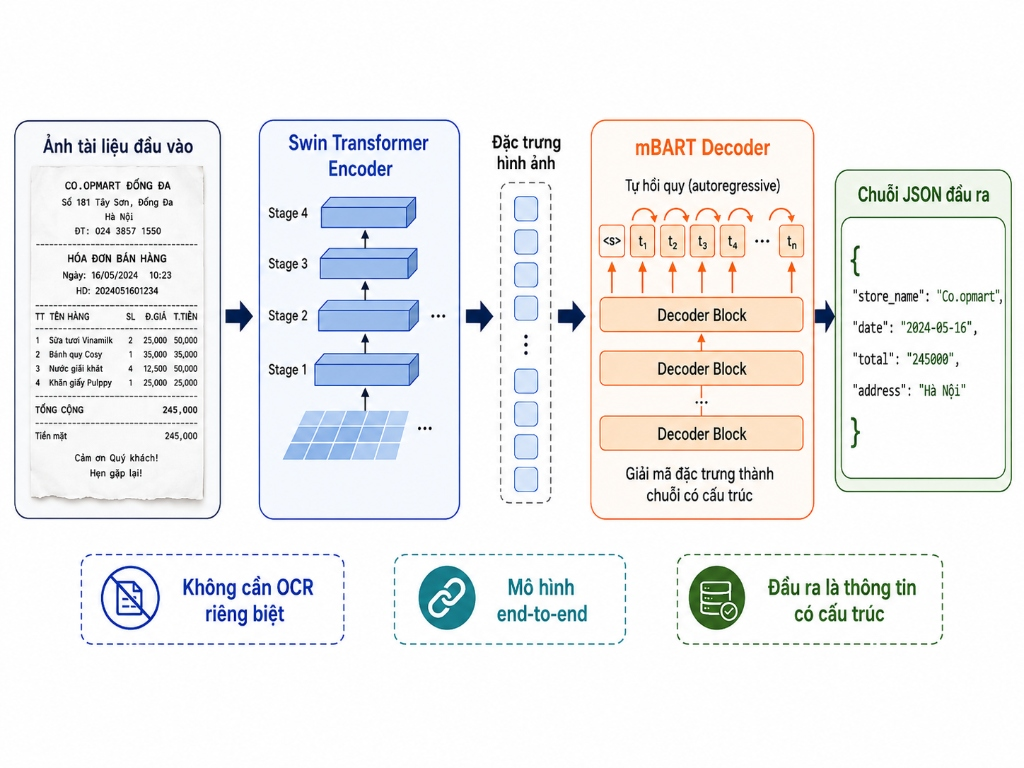
\includegraphics[width=0.85\textwidth]{donut_architecture.jpg}
  \caption{Kiến trúc tổng quan mô hình \model{Donut} (Swin Encoder kết hợp mBART Decoder)~\cite{kim2022donut}.}
  \label{fig:donut_arch}
\end{figure}

\subsubsection{Phân biệt khái niệm Warm-up trong Donut}
\label{subsubsec:donut_warmup}

Trong quá trình huấn luyện mô hình Donut, cần phân biệt rõ hai khái niệm "warm-up" dễ gây nhầm lẫn:
\begin{itemize}
  \item \textbf{Learning Rate Warm-up (tỷ lệ $warmup\_ratio$ hoặc số bước $warmup\_steps$):} Đây là một kỹ thuật điều tiết tốc độ học trong tối ưu hóa (LR scheduling). Trong số bước đầu tiên (thường là 10\% tổng số bước huấn luyện), tốc độ học được tăng dần tuyến tính từ 0 lên mức cực đại được thiết lập nhằm tránh hiện tượng bùng nổ gradient khi bắt đầu cập nhật trọng số.
  \item \textbf{Pre-training/Warm-up mô hình trên tập CORD:} Đây là một bước huấn luyện phụ (pre-finetuning). Trước khi huấn luyện trên tập dữ liệu biên lai tiếng Việt chính, mô hình Donut được huấn luyện trên một tập dữ liệu biên lai lớn khác (như CORD v2 gồm 800 mẫu tiếng Anh) để mô hình làm quen với bố cục và cấu trúc biểu diễn thẻ XML tổng quát của biên lai.
\end{itemize}

% ============================================================================
\subsection{Mô hình LayoutXLM (OCR-based)}
\label{subsec:layoutxlm}

\model{LayoutXLM}~\cite{xu2021layoutxlm} là mô hình đa phương thức đa ngôn ngữ tiền huấn luyện dành riêng cho các tài liệu có cấu trúc bố cục phong phú, kế thừa backbone XLM-RoBERTa~\cite{conneau2020xlmr}.

\subsubsection{Nhúng đa phương thức (Multimodal Embedding)}
\label{subsubsec:multimodal_embedding}

Để biểu diễn một token văn bản trong tài liệu, LayoutXLM kết hợp ba loại vector nhúng:
\begin{enumerate}
  \item \textbf{Nhúng văn bản (Text Embedding):} Mã hóa đặc trưng ngữ nghĩa của từ.
  \item \textbf{Nhúng không gian 2D (Spatial Embedding):} Tọa độ bounding box $[x_1, y_1, x_2, y_2]$ của từ được chuẩn hóa về khoảng $[0, 1000]$ và nhúng thông qua các bảng nhúng tọa độ để mô hình nắm bắt vị trí tương đối và tuyệt đối trên ảnh:
  \begin{equation}
    \mathbf{e}_{2D}(\text{bbox}_i) = \mathbf{e}_{x_1}(x_1) + \mathbf{e}_{y_1}(y_1) + \mathbf{e}_{x_2}(x_2) + \mathbf{e}_{y_2}(y_2) + \mathbf{e}_{w}(w) + \mathbf{e}_{h}(h)
  \end{equation}
  \item \textbf{Nhúng thị giác (Visual Embedding):} Cắt vùng ảnh tương ứng với bounding box của token và đưa qua mạng CNN (ResNeXt) để trích xuất đặc trưng hình ảnh (phông chữ, độ đậm nhạt, màu sắc).
\end{enumerate}

Vector biểu diễn tổng hợp của token là tổng của ba thành phần trên: $\mathbf{x}_i = \mathbf{t}_i + \mathbf{e}_{2D}(\text{bbox}_i) + \mathbf{v}_i$.

\subsubsection{Spatial-aware Self-Attention}
\label{subsubsec:spatial_attention}

Cơ chế tự chú ý nhận biết không gian (spatial-aware) của LayoutXLM bổ sung thêm các thông tin thiên lệch vị trí (bias) theo chiều dọc và chiều ngang dựa trên khoảng cách vật lý giữa hai bounding box của token $i$ và token $j$:
\begin{equation}
  \alpha_{ij} = \frac{\mathbf{q}_i \mathbf{k}_j^T}{\sqrt{d}} + b^{1D}(j - i) + b^{2D}_x(x_{1,i} - x_{1,j}) + b^{2D}_y(y_{1,i} - y_{1,j})
\end{equation}
Điều này giúp mô hình tự động học được mối liên hệ logic giữa các từ nằm gần nhau về mặt không gian địa lý trên ảnh tài liệu.

\subsubsection{Gán nhãn BIO (BIO Tagging)}
\label{subsubsec:bio_tagging}

Để thực hiện trích xuất thông tin, bài toán được định nghĩa dưới dạng phân loại token (token classification). Mỗi token đầu vào được dự đoán một nhãn trong hệ thống nhãn \gls{bio} gồm 9 nhãn được mô tả chi tiết trong \cref{tab:bio_labels}.

\begin{table}[htbp]
  \centering
  \caption{Hệ thống nhãn \gls{bio} cho 4 trường thông tin trích xuất.}
  \label{tab:bio_labels}
  \begin{tabular}{lll}
    \toprule
    \textbf{Trường thông tin} & \textbf{Nhãn Bắt đầu (Begin)} & \textbf{Nhãn Bên trong (Inside)} \\
    \midrule
    Tên cửa hàng (\field{store\_name}) & \texttt{B-STORE\_NAME} & \texttt{I-STORE\_NAME} \\
    Ngày tháng (\field{date})           & \texttt{B-DATE}        & \texttt{I-DATE}        \\
    Tổng tiền (\field{total})           & \texttt{B-TOTAL}       & \texttt{I-TOTAL}       \\
    Địa chỉ (\field{address})           & \texttt{B-ADDRESS}     & \texttt{I-ADDRESS}     \\
    Trường không quan tâm               & \multicolumn{2}{l}{\texttt{O} (Outside)} \\
    \bottomrule
  \end{tabular}
\end{table}

% ============================================================================
\subsection{Các độ đo đánh giá và quy ước xử lý rỗng}
\label{subsec:metrics}

Để đánh giá chính xác chất lượng trích xuất, các dự đoán sau khi được chuẩn hóa sẽ được so sánh với nhãn ground-truth thông qua ba chỉ số chính: EM, NES, và CER. 

\subsubsection{Exact Match (EM)}
EM đo tỷ lệ khớp chính xác hoàn toàn từng ký tự giữa dự đoán ($pred$) và nhãn thực ($gold$):
\begin{equation}
  \metric{EM}(pred, gold) = \begin{cases} 
    1.0 & \text{nếu } pred.strip() = gold.strip() \\
    0.0 & \text{ngược lại}
  \end{cases}
\end{equation}
\textbf{Quy ước giá trị rỗng:} Nếu cả $pred$ và $gold$ đều là chuỗi rỗng sau chuẩn hóa $\to \metric{EM} = 1.0$. Nếu chỉ một trong hai chuỗi rỗng $\to \metric{EM} = 0.0$.

\subsubsection{Normalized Edit Similarity (NES)}
NES đo mức độ tương đồng ngữ nghĩa ký tự thông qua khoảng cách Levenshtein chuẩn hóa:
\begin{equation}
  \metric{NES}(pred, gold) = 1 - \frac{\text{Levenshtein}(pred, gold)}{\max(\text{len}(pred), \text{len}(gold))}
\end{equation}
\textbf{Quy ước giá trị rỗng:} Nếu cả $pred$ và $gold$ đều là chuỗi rỗng $\to \metric{NES} = 1.0$ (tránh lỗi chia cho 0). Nếu chỉ một trong hai chuỗi rỗng $\to \metric{NES} = 0.0$.

\subsubsection{Character Error Rate (CER)}
CER đo tỷ lệ lỗi ở cấp độ ký tự trên chuỗi nhãn thực:
\begin{equation}
  \metric{CER}(pred, gold) = \frac{\text{Levenshtein}(pred, gold)}{\text{len}(gold)}
\end{equation}
\textbf{Quy ước giá trị rỗng:} 
\begin{itemize}
  \item Nếu cả hai cùng rỗng $\to \metric{CER} = 0.0$.
  \item Nếu $gold$ rỗng nhưng $pred$ có giá trị $\to \metric{CER} = 1.0$.
  \item Nếu $gold$ có giá trị nhưng $pred$ rỗng $\to \metric{CER} = 1.0$.
\end{itemize}
\textbf{Giải thích hiện tượng CER > 100\%:} Chỉ số CER có thể vượt quá 100\% (hay > 1.0) khi chuỗi dự đoán dài hơn đáng kể so với nhãn thực do mô hình sinh thừa nhiều ký tự rác hoặc bị lỗi lặp chuỗi tự hồi quy (hallucination), dẫn đến khoảng cách Levenshtein lớn hơn độ dài ký tự của nhãn thực $gold$.

\newpage
% ============================================================================
%  CHƯƠNG 3 — Thu thập và xây dựng tập dữ liệu
% ============================================================================

\section{Thu thập và xây dựng tập dữ liệu}
\label{sec:dataset}

Chương này mô tả chi tiết quy trình thu thập dữ liệu từ các nguồn khác nhau, xây dựng hướng dẫn gán nhãn chuẩn hóa và schema lưu trữ JSONL thống nhất. Đồng thời, chương trình bày chi tiết quy trình lọc dữ liệu từ ảnh thô sang tập dữ liệu sạch, các biện pháp kỹ thuật chống rò rỉ thông tin (data leakage) và thống kê tỷ lệ thiếu nhãn.

% ----------------------------------------------------------------------------
\subsection{Nguồn dữ liệu và quy trình lọc mẫu}
\label{subsec:data-source}

Đồ án kết hợp hai nguồn dữ liệu biên lai tiếng Việt: bộ dữ liệu công khai từ cuộc thi MC-OCR 2021 và bộ dữ liệu tự chụp thực tế từ các cửa hàng bán lẻ khác nhau. Quy trình hình thành tập dữ liệu sạch trải qua các bước lọc nghiêm ngặt được tổng hợp trong \cref{tab:data-filtering-stats}.

\subsubsection{MC-OCR 2021}
Tập dữ liệu gốc từ cuộc thi \gls{mcocr} 2021~\cite{mcocr2021} bao gồm \textbf{2.436 ảnh} biên lai. Tuy nhiên, tập dữ liệu này chứa cả phần public test không đi kèm nhãn ground-truth. Nhóm nghiên cứu chỉ lọc và sử dụng phần dữ liệu huấn luyện có nhãn đầy đủ gồm \textbf{1.094 mẫu}. 

Nhãn gốc của MC-OCR được ánh xạ sang schema thống nhất của đồ án như sau:
\begin{itemize}
  \item \code{SELLER} $\to$ \field{store\_name} (Tên cửa hàng)
  \item \code{SELLER\_ADDRESS} $\to$ \field{address} (Địa chỉ)
  \item \code{TIMESTAMP} $\to$ \field{date} (Ngày giao dịch)
  \item \code{TOTAL\_COST} $\to$ \field{total} (Tổng số tiền thanh toán)
\end{itemize}

\subsubsection{Dữ liệu tự thu thập}
Để tăng tính đa dạng và kiểm định tính thực tiễn, nhóm nghiên cứu tự chụp thêm \textbf{500 ảnh} biên lai thực tế từ siêu thị, nhà hàng, cửa hàng tiện lợi tại Hà Nội. Các hình ảnh được chụp bằng thiết bị di động trong điều kiện ánh sáng, góc chụp biến động mạnh và ảnh có thể bị nghiêng, mờ nhẹ. Việc gán nhãn được thực hiện thủ công bằng công cụ Label Studio\footnote{\url{https://labelstud.io}} để đánh dấu bounding box và nhập giá trị văn bản cho 4 trường thông tin.

\subsubsection{Quy trình lọc trùng lặp ảnh (MD5 Deduplication)}
Nhằm loại bỏ các ảnh trùng lặp hoặc các ảnh chụp cùng một hóa đơn nhiều lần nhưng ở các góc máy gần tương tự nhau, nhóm nghiên cứu chạy thuật toán băm MD5 kiểm tra nội dung ảnh trước khi phân chia dữ liệu:
1. Tính giá trị băm MD5 cho từng tệp ảnh.
2. Nếu phát hiện tệp ảnh có cùng mã MD5 với tệp đã xử lý trước đó, tệp ảnh này sẽ bị loại khỏi tập dữ liệu.
Quy trình này đã phát hiện và loại bỏ \textbf{98 mẫu ảnh trùng lặp} (gồm 63 mẫu từ MC-OCR và 35 mẫu tự chụp).

\begin{table}[htbp]
  \centering
  \caption{Thống kê số lượng mẫu bị loại theo từng nguồn dữ liệu.}
  \label{tab:data-filtering-stats}
  \begin{tabular}{lcccc}
    \toprule
    \textbf{Nguồn dữ liệu} & \textbf{Ảnh thô ban đầu} & \textbf{Loại do thiếu nhãn} & \textbf{Loại do trùng MD5} & \textbf{Mẫu sạch cuối cùng} \\
    \midrule
    MC-OCR 2021 & 2.436 & 1.279 & 63 & 1.094 \\
    Tự thu thập  & 500   & 0     & 35 & 465   \\
    \midrule
    \textbf{Tổng} & \textbf{2.936} & \textbf{1.279} & \textbf{98} & \textbf{1.559} \\
    \bottomrule
  \end{tabular}
\end{table}

% ----------------------------------------------------------------------------
\subsection{Hướng dẫn gán nhãn (Annotation Guideline) và QA/QC}
\label{subsec:annotation-guideline}

Việc gán nhãn dữ liệu tuân thủ nghiêm ngặt bộ quy tắc chuẩn hóa nhằm bảo đảm tính nhất quán cao nhất giữa các nguồn dữ liệu khác nhau:
\begin{itemize}
  \item \field{store\_name}: Chỉ lấy tên thương hiệu/cửa hàng chính thức, loại bỏ các loại hình kinh doanh như "Công ty TNHH", "Cửa hàng bán lẻ" hoặc MST đi kèm.
  \item \field{date}: Chỉ lấy thông tin ngày tháng năm và chuẩn hóa về định dạng YYYY-MM-DD. Loại bỏ các tiền tố như "Ngày:", "Giờ:", hoặc thông tin giờ phút giây.
  \item \field{total}: Chỉ lấy số tiền thanh toán cuối cùng (final payment), loại bỏ đơn vị tiền tệ, dấu phân cách hàng nghìn và các số 0 ở đầu. Không lấy giá trị tạm tính (subtotal) hoặc tiền thừa (change).
  \item \field{address}: Lấy toàn bộ địa chỉ ghi trên biên lai, loại bỏ số điện thoại, website, email đi kèm.
\end{itemize}

\textbf{Quy trình QA/QC (Kiểm soát chất lượng):} 
Sau khi hoàn tất gán nhãn tự chụp, nhóm tiến hành kiểm soát chất lượng ngẫu nhiên trên \textbf{50 mẫu}. Kết quả QA/QC ghi nhận tỷ lệ sai lệch ban đầu là 8.0\% (4 mẫu), chủ yếu liên quan đến việc nhầm lẫn giữa trường \field{total} và subtotal, hoặc gán nhãn địa chỉ bị thiếu dòng. Toàn bộ sai lệch phát hiện đều được nhóm nghiên cứu tiến hành sửa đổi thủ công để đạt độ chính xác nhãn sạch 100\% trước khi chuyển qua bước huấn luyện.

% ============================================================================
\subsection{Schema dữ liệu thống nhất (Unified JSONL)}
\label{subsec:unified-schema}

Toàn bộ dữ liệu sạch từ cả hai nguồn được chuyển đổi về một schema JSONL thống nhất với \textbf{13 trường chính} được mô tả chi tiết trong \cref{tab:jsonl-schema}.

\begin{table}[htbp]
  \centering
  \caption{Mô tả 13 trường dữ liệu trong schema JSONL thống nhất.}
  \label{tab:jsonl-schema}
  \begin{tabularx}{\textwidth}{lL{9.5cm}}
    \toprule
    \textbf{Trường} & \textbf{Mô tả} \\
    \midrule
    \code{id}                & Mã định danh duy nhất của mỗi mẫu ảnh \\
    \code{group\_id}         & Mã nhóm ảnh (dùng để nhận diện các ảnh chụp cùng biên lai) \\
    \code{store\_group}      & Tên nhóm cửa hàng (phục vụ phân tầng và stress-test) \\
    \code{source}            & Nguồn dữ liệu (\code{mc\_ocr\_2021} hoặc \code{self\_collected}) \\
    \code{image\_path}       & Đường dẫn tương đối đến tệp ảnh \\
    \code{width}             & Chiều rộng ảnh gốc (pixel) \\
    \code{height}            & Chiều cao ảnh gốc (pixel) \\
    \code{annotation\_level} & Mức độ chú thích (\code{json\_and\_boxes} hoặc \code{json\_only}) \\
    \code{raw\_target}       & Nhãn thô ban đầu trước chuẩn hóa (JSON object) \\
    \code{target}            & Nhãn sạch đã qua chuẩn hóa (JSON object) \\
    \code{field\_boxes}      & Tọa độ bounding box $[x_1, y_1, x_2, y_2]$ của từng trường \\
    \code{field\_polygons}   & Tọa độ đa giác của từng trường thông tin \\
    \code{ocr\_cache\_path}  & Đường dẫn đến tệp lưu kết quả OCR cache \\
    \bottomrule
  \end{tabularx}
\end{table}

Ví dụ một dòng dữ liệu trong tệp JSONL thống nhất:
\begin{lstlisting}[style=json, caption={Ví dụ một dòng dữ liệu JSONL}, label={lst:jsonl-example}]
{
  "id": "mcocr_0001",
  "group_id": "g_0001",
  "store_group": "circlek",
  "source": "mcocr",
  "image_path": "images/mcocr_0001.jpg",
  "width": 1080, "height": 1920,
  "annotation_level": "json_and_boxes",
  "raw_target": {
    "store_name": "CIRCLE K",
    "address": "123 Nguyen Trai, HN",
    "date": "15/03/2021",
    "total": "115.000"
  },
  "target": {
    "store_name": "circle k",
    "address": "123 nguyen trai, hn",
    "date": "2021-03-15",
    "total": "115000"
  },
  "field_boxes": {"store_name": [100, 50, 400, 90]},
  "field_polygons": {},
  "ocr_cache_path": "ocr_cache/mcocr_0001.json"
}
\end{lstlisting}

% ============================================================================
\subsection{Chiến lược chia dữ liệu (Data Split) và ngăn ngừa Leakage}
\label{subsec:data-split}

\paragraph{Rủi ro rò rỉ dữ liệu (Data Leakage)}
Trong bài toán trích xuất thông tin biên lai, hiện tượng rò rỉ dữ liệu xảy ra khi các hình ảnh chụp cùng một biên lai vật lý (nhưng ở các góc máy khác nhau) bị phân chia nằm ở cả hai tập huấn luyện (Train) và tập kiểm thử (Test). Điều này làm cho mô hình dễ dàng "ghi nhớ" bố cục và nội dung cụ thể, dẫn đến kết quả đánh giá bị sai lệch và không phản ánh đúng khả năng tổng quát hóa thực tế của mô hình.

\paragraph{Biện pháp giải quyết trong Đồ án}
Để loại bỏ triệt để nguy cơ rò rỉ dữ liệu, nhóm nghiên cứu thiết lập chiến lược phân chia Main Split tỷ lệ \textbf{70/15/15} (Train/Val/Test) với hai ràng buộc kỹ thuật nghiêm ngặt:
1. \textbf{Group-based Split:} Việc phân chia được thực hiện ở cấp độ `group_id` (chứ không phải cấp tệp ảnh đơn lẻ). Toàn bộ ảnh có chung `group_id` bắt buộc phải nằm trong cùng một tập (hoặc Train, hoặc Val, hoặc Test).
2. \textbf{MD5 Hash Check:} Việc kiểm tra mã băm MD5 đảm bảo không có bất kỳ ảnh nào giống hệt nhau tồn tại song song giữa các tập split.
3. \textbf{Phân tầng theo nguồn (Stratified by source):} Đảm bảo tỷ lệ phân bố giữa dữ liệu MC-OCR và dữ liệu tự chụp là tương đương giữa các tập huấn luyện, phát triển và kiểm thử.

Thống kê số lượng mẫu sau phân chia được trình bày trong \cref{tab:split-stats}.

\begin{table}[htbp]
  \centering
  \caption{Phân bố số lượng mẫu sạch theo các tập dữ liệu.}
  \label{tab:split-stats}
  \begin{tabular}{lccc}
    \toprule
    \textbf{Tập dữ liệu} & \textbf{MC-OCR 2021} & \textbf{Tự thu thập} & \textbf{Tổng số mẫu} \\
    \midrule
    Train (Huấn luyện) & 766 & 325 & 1.091 \\
    Val (Phát triển)   & 164 & 70  & 234   \\
    Test (Kiểm thử)    & 164 & 70  & 234   \\
    \midrule
    \textbf{Tổng} & \textbf{1.094} & \textbf{465} & \textbf{1.559} \\
    \bottomrule
  \end{tabular}
\end{table}

\paragraph{Thống kê tỷ lệ thiếu nhãn trên tập kiểm thử (Test Set)}
Trong thực tế, một số biên lai bị thiếu thông tin hoặc thông tin bị mờ không thể đọc được. \cref{tab:missing-rate} thống kê số mẫu thiếu nhãn (missing rate) của từng trường cụ thể trên tập kiểm thử (Test set) gồm \textbf{234 mẫu}, phản ánh độ thử thách của tập kiểm định thực tế.

\begin{table}[htbp]
  \centering
  \caption{Tỷ lệ thiếu nhãn theo từng trường trên tập kiểm thử (234 mẫu).}
  \label{tab:missing-rate}
  \begin{tabular}{lcc}
    \toprule
    \textbf{Trường thông tin} & \textbf{Số mẫu thiếu nhãn} & \textbf{Tỷ lệ thiếu (\%)} \\
    \midrule
    \field{store\_name} & 10 & 4,27\% \\
    \field{date}        & 18 & 7,69\% \\
    \field{total}       & 17 & 7,26\% \\
    \field{address}     & 11 & 4,70\% \\
    \bottomrule
  \end{tabular}
\end{table}

% ============================================================================
\subsection{Kiểm tra tính hợp lệ dữ liệu (Validation)}
\label{subsec:data-validation}

Trước khi đưa vào huấn luyện, toàn bộ 1.559 mẫu dữ liệu sạch được chạy qua script tự động \code{validate\_dataset} để xác minh cú pháp và định dạng nhãn. Script thực hiện kiểm tra:
\begin{itemize}
  \item Định dạng ngày \field{date} phải tuân thủ chuẩn ISO \code{YYYY-MM-DD}.
  \item Giá trị trường \field{total} phải là chuỗi số nguyên thuần túy (không chứa ký tự chữ cái, đơn vị tiền tệ hoặc dấu phân cách hàng nghìn).
  \item Đường dẫn \code{image\_path} phải hợp lệ và tệp ảnh không bị lỗi đọc ghi (corrupted image).
\end{itemize}

Kết quả chạy thử nghiệm ghi nhận 15 mẫu có lỗi định dạng ngày tháng (chứa ký tự giờ phút giây ở nhãn chuẩn hóa) và 8 mẫu có trường \field{total} chứa dấu phân cách hàng nghìn. Nhóm nghiên cứu đã khắc phục triệt để các lỗi này bằng cách tinh chỉnh các bộ lọc chuẩn hóa văn bản tự động, đưa tỷ lệ lỗi hợp lệ về 0\% trước khi chính thức huấn luyện.

\newpage
% ============================================================================
%  CHƯƠNG 4 — Tiền xử lý dữ liệu
% ============================================================================

\section{Tiền xử lý dữ liệu}
\label{sec:preprocessing}

Chương này trình bày các bước xử lý hình ảnh và văn bản nhằm tối ưu hóa chất lượng đầu vào cho các mô hình trích xuất. Nội dung tập trung phân biệt các kỹ thuật tiền xử lý áp dụng thực tế với các kỹ thuật chỉ dùng khảo sát thử nghiệm, chi tiết hóa quy tắc chuẩn hóa văn bản, và phân tích thí nghiệm ablation lựa chọn cấu hình xử lý ảnh tối ưu cho bộ OCR.

% ============================================================================
\subsection{Tiền xử lý ảnh (Image Preprocessing)}
\label{subsec:image-preprocessing}

Chất lượng ảnh biên lai đầu vào ảnh hưởng trực tiếp đến hiệu năng nhận dạng của bộ OCR. Nhóm nghiên cứu chia các kỹ thuật xử lý ảnh làm hai nhóm rõ rệt:

\paragraph{1. Kỹ thuật tiền xử lý áp dụng thực tế (Production Pipeline)}
Đây là các bước bắt buộc được tích hợp trong luồng xử lý chính thức của hệ thống:
\begin{itemize}
  \item \textbf{Resize hình ảnh:} 
  \begin{itemize}
    \item Đối với pipeline OCR (Baseline và LayoutXLM): Ảnh được resize theo cạnh dài nhất với $\text{max\_long\_side} = 1600$ pixel để bảo đảm nét chữ rõ ràng và duy trì tỷ lệ khung hình (aspect ratio).
    \item Đối với Donut: Ảnh được resize về kích thước cố định $1280 \times 960$ pixel, phần thiếu được lấp đầy bằng khoảng trắng (padding).
  \end{itemize}
  \item \textbf{Khử nhiễu (Denoise):} Áp dụng bộ lọc Non-local Means Denoising để loại bỏ nhiễu hạt sinh ra do điều kiện chụp thiếu sáng.
  \item \textbf{Cân bằng tương phản CLAHE:} Cân bằng histogram thích ứng giới hạn độ tương phản (Contrast Limited Adaptive Histogram Equalization) để xử lý các vùng ảnh bị phản quang hoặc có độ sáng không đều.
\end{itemize}

\paragraph{2. Kỹ thuật khảo sát thử nghiệm (Ablation Only)}
Đây là các kỹ thuật chỉ được khảo sát trong thí nghiệm ablation để đánh giá tác động định lượng, không được đưa vào pipeline vận hành thực tế do gây suy giảm chất lượng hoặc tốn nhiều thời gian xử lý:
\begin{itemize}
  \item \textbf{Nhị phân hóa (Binarize):} Áp dụng thuật toán nhị phân hóa Otsu để chuyển ảnh về định dạng đen trắng tuyệt đối.
  \item \textbf{Nắn thẳng ảnh (Rectify):} Sử dụng phép biến đổi affine để xoay và nắn thẳng các ảnh biên lai bị nghiêng hoặc chụp lệch góc.
\end{itemize}

% ============================================================================
\subsection{Tăng cường dữ liệu (Data Augmentation)}
\label{subsec:augmentation}

Nhằm nâng cao khả năng tổng quát hóa của mô hình học sâu và chống quá khớp (overfitting), nhóm nghiên cứu áp dụng các kỹ thuật tăng cường dữ liệu hình ảnh trực tuyến (online augmentation) \textbf{chỉ trên tập huấn luyện (Train set)}. Cấu hình chi tiết được mô tả trong \cref{tab:augmentation}.

\begin{table}[htbp]
  \centering
  \caption{Các thông số kỹ thuật tăng cường dữ liệu trong quá trình huấn luyện.}
  \label{tab:augmentation}
  \begin{tabular}{llc}
    \toprule
    \textbf{Kỹ thuật tăng cường} & \textbf{Tham số thiết lập} & \textbf{Xác suất áp dụng (p)} \\
    \midrule
    Xoay ảnh (Rotate)           & Biên độ $\pm 2^{\circ}$     & 0,40 \\
    Thay đổi độ sáng/tương phản  & Biên độ $\pm 0,2$          & 0,40 \\
    Nén ảnh JPEG (Compression)  & Chất lượng $60\% - 100\%$   & 0,30 \\
    Làm mờ Gauss (Gaussian Blur)& Bộ lọc kích thước $3 \times 3$ & 0,15 \\
    Phép biến đổi phối cảnh     & Tỷ lệ biến đổi $0,01 - 0,03$& 0,20 \\
    \bottomrule
  \end{tabular}
\end{table}

% ============================================================================
\subsection{Chuẩn hoá văn bản (Text Normalization)}
\label{subsec:text-normalization}

Chuẩn hóa văn bản là bước bắt buộc để đồng nhất định dạng dữ liệu đầu ra và sửa các lỗi chính tả nhỏ do bộ gõ tiếng Việt gây ra. Quy trình chuẩn hóa gồm hai bước:

\paragraph{1. Chuẩn hóa chung (General Normalization)}
Áp dụng cho toàn bộ các trường thông tin:
\begin{itemize}
  \item \textbf{Unicode NFC:} Chuyển đổi toàn bộ văn bản về dạng chuẩn tổ hợp Unicode NFC để đồng nhất biểu diễn ký tự có dấu.
  \item \textbf{Whitespace:} Gộp các khoảng trắng liên tiếp và cắt khoảng trắng ở hai đầu chuỗi.
  \item \textbf{Ký tự đặc biệt:} Loại bỏ các ký tự điều khiển không in được.
\end{itemize}

\paragraph{2. Chuẩn hóa theo trường (Field-specific Normalization)}
\begin{itemize}
  \item \field{store\_name}: Loại bỏ các tiền tố pháp lý hoặc loại hình kinh doanh (ví dụ: "Cửa hàng", "Siêu thị", "Công ty", "TNHH").
  \item \field{address}: Loại bỏ các tiền tố địa chỉ như "Địa chỉ:", "Đ/c:", "ĐC:".
  \item \field{date}: Chuyển đổi nhiều định dạng ngày tự do về dạng chuẩn ISO \code{YYYY-MM-DD}. Nếu phân tích cú pháp thất bại, trả về chuỗi rỗng.
  \item \field{total}: Loại bỏ đơn vị tiền tệ ("đ", "đồng", "VND"), dấu chấm/phẩy phân cách hàng nghìn và các số 0 ở đầu.
\end{itemize}

\cref{tab:normalization-examples} minh họa kết quả chuẩn hóa cho từng trường.

\begin{table}[htbp]
  \centering
  \caption{Ví dụ chuẩn hoá văn bản theo trường thông tin.}
  \label{tab:normalization-examples}
  \begin{tabularx}{\textwidth}{lL{5cm}L{5cm}}
    \toprule
    \textbf{Trường} & \textbf{Văn bản gốc trước chuẩn hóa} & \textbf{Văn bản sau chuẩn hóa} \\
    \midrule
    \field{store\_name} & Cửa hàng tiện lợi CIRCLE K & circle k \\
    \field{address}     & Địa chỉ: 123 Nguyễn Trãi, Thanh Xuân, HN & 123 nguyen trai, thanh xuan, hn \\
    \field{date}        & Lúc 15/03/2021 14:30:15 & 2021-03-15 \\
    \field{total}       & Tổng cộng: 115.000 đ & 115000 \\
    \bottomrule
  \end{tabularx}
\end{table}

% ============================================================================
\subsection{Xây dựng OCR Cache}
\label{subsec:ocr-cache}

Quá trình chạy mô hình OCR (PaddleOCR kết hợp VietOCR) tốn nhiều tài nguyên tính toán và thời gian. Việc xây dựng OCR cache giúp lưu trữ lại kết quả nhận diện của từng ảnh để sử dụng lại tức thì trong các lượt huấn luyện và thực nghiệm khác nhau, đẩy nhanh đáng kể tốc độ thử nghiệm.

Hệ thống đã xây dựng OCR cache thành công cho toàn bộ 1.559 mẫu ảnh trong tập dữ liệu. Tổng dung lượng cache chiếm khoảng 12,4 MB dưới dạng tệp tin JSON. Thời gian chạy OCR trung bình cho mỗi ảnh biên lai là 1,12 giây trên CPU và 0,18 giây khi sử dụng GPU tăng tốc.

% ============================================================================
\subsection{Thí nghiệm Ablation tiền xử lý ảnh cho OCR}
\label{subsec:ocr-ablation}

\paragraph{1. Định nghĩa Metric ``OCR Quality''}
Để đánh giá định lượng chất lượng của kết quả OCR thô sau các bước tiền xử lý ảnh mà không phụ thuộc vào luật trích xuất, nhóm nghiên cứu đề xuất chỉ số \textbf{OCR Quality}. Chỉ số này được tính toán như sau:
\begin{itemize}
  \item Đối với mỗi mẫu ảnh, kết quả nhận dạng OCR của tất cả các hộp bao chữ được ghép nối phẳng cách nhau bởi dấu cách tạo thành chuỗi văn bản $ocr\_text$.
  \item Tiến hành chuẩn hóa loại bỏ dấu tiếng Việt, chuyển chữ thường và loại bỏ toàn bộ ký tự đặc biệt trên cả chuỗi $ocr\_text$ và chuỗi nhãn thực $gold$ của 4 trường thông tin trích xuất.
  \item Tính điểm độ tương đồng chuỗi con mờ (partial fuzzy match ratio - $\text{partial\_ratio}$) giữa chuỗi thực tế và chuỗi OCR phẳng:
\end{itemize}
  \begin{equation}
    \text{Score}(field) = \frac{\text{partial\_ratio}(gold\_normalized, ocr\_text\_normalized)}{100.0}
  \end{equation}
\begin{itemize}
  \item Nếu nhãn thực của trường đó trống, gán $\text{Score} = 1.0$.
  \item Điểm ``OCR Quality'' của mẫu ảnh là trung bình cộng của 4 trường thông tin. Điểm tổng thể của profile tiền xử lý là trung bình cộng điểm của toàn bộ các mẫu ảnh được kiểm tra.
\end{itemize}

\paragraph{2. Thiết lập tập dữ liệu ablation và nguyên tắc bảo vệ tập kiểm thử}
Để bảo đảm tính trung thực khoa học, toàn bộ thí nghiệm ablation tiền xử lý ảnh được thực hiện trên \textbf{100 mẫu ngẫu nhiên được trích xuất từ tập Validation (val.jsonl)}. 

Nhóm nghiên cứu \textbf{hoàn toàn không sử dụng tập kiểm thử (Test set)} để lựa chọn cấu hình tiền xử lý. Nguyên tắc này giúp ngăn ngừa hiện tượng rò rỉ dữ liệu hoặc tinh chỉnh thiên vị (overfitting) cấu hình xử lý lên tập test độc lập, bảo đảm kết quả đánh giá cuối cùng phản ánh chính xác khả năng tổng quát hóa thực tế của toàn bộ hệ thống.

Kết quả thí nghiệm ablation được tổng hợp trong \cref{tab:ocr-ablation}.

\begin{table}[htbp]
  \centering
  \caption{Kết quả thí nghiệm ablation tiền xử lý ảnh trên 100 mẫu Validation.}
  \label{tab:ocr-ablation}
  \begin{tabular}{lc}
    \toprule
    \textbf{Cấu hình tiền xử lý (Profile)} & \textbf{OCR Quality (\%)} \\
    \midrule
    \textbf{none} (Ảnh gốc, không tiền xử lý) & 78,50 \\
    \textbf{resize} (Resize $\text{max\_long\_side} = 1600$, denoise, clahe) & \textbf{84,32} \\
    \textbf{binarize} (Otsu binarization) & 81,15 \\
    \textbf{rectify} (Affine rectification) & 82,68 \\
    \bottomrule
  \end{tabular}
\end{table}

\paragraph{3. Phân tích kết quả}
Kết quả cho thấy cấu hình \textbf{resize} kết hợp khử nhiễu và CLAHE mang lại hiệu năng cao nhất (84,32\%), cải thiện rõ rệt so với ảnh gốc (78,50\%). 
\begin{itemize}
  \item Kỹ thuật nhị phân hóa Otsu cứng làm mất chi tiết nét chữ mảnh trên giấy in nhiệt bị mờ, dẫn đến chất lượng nhận dạng giảm xuống còn 81,15\%.
  \item Phép nắn thẳng ảnh (rectify) tuy cải thiện so với không xử lý nhưng vẫn kém hơn profile resize thông thường do thuật toán phát hiện góc nghiêng tự động đôi khi ước lượng sai lệch, gây méo cục bộ ảnh chữ viết.
\end{itemize}

Do đó, cấu hình \textbf{resize} được lựa chọn làm cấu hình tiền xử lý chính thức trong toàn bộ pipeline thực nghiệm tiếp theo.

\newpage
% ============================================================================
%  SECTION 5 — Phương pháp thực hiện
% ============================================================================
\section{Phương pháp thực hiện}
\label{sec:methodology}

% >>> BẢN NHÁP: Giới thiệu chương (Sinh viên đọc lại và chỉnh sửa) <<<
Chương này trình bày chi tiết thiết kế hệ thống và phương pháp thực hiện của ba hướng tiếp cận (pipeline) khác nhau nhằm giải quyết bài toán trích xuất thông tin biên lai tiếng Việt, bao gồm phương pháp Baseline dựa trên biểu thức chính quy, mô hình sinh End-to-End Donut, và mô hình phân loại chuỗi LayoutXLM kết hợp nhận dạng văn bản VietOCR.

% ============================================================================
\subsection{Tổng quan kiến trúc hệ thống}
\label{subsec:system_overview}

% >>> BẢN NHÁP: Giới thiệu hệ thống (Sinh viên đọc lại và chỉnh sửa) <<<
Hệ thống được thiết kế dạng module hóa cho phép kiểm thử và so sánh độc lập các kiến trúc. Sơ đồ kiến trúc tổng quan của ba phương pháp được mô tả chi tiết trong Hình 5.1 dưới đây.
Hệ thống nhận đầu vào là ảnh biên lai và đầu ra là tệp JSON chứa bốn trường thông tin:
\field{store\_name}, \field{date}, \field{total}, \field{address}.

\begin{itemize}
  \item \textbf{Pipeline 1 — Baseline (Rule-based):}
    Ảnh $\rightarrow$ \gls{ocr} (PaddleOCR + VietOCR) $\rightarrow$
    Luật / Regex $\rightarrow$ JSON.

  \item \textbf{Pipeline 2 — \model{Donut} (OCR-free):}
    Ảnh $\rightarrow$ Swin Encoder $\rightarrow$ \gls{bart} Decoder
    $\rightarrow$ JSON.

  \item \textbf{Pipeline 3 — VietOCR + \model{LayoutXLM} (OCR-based):}
    Ảnh $\rightarrow$ \gls{ocr} $\rightarrow$ Token + BBox $\rightarrow$
    \model{LayoutXLM} $\rightarrow$ \gls{bio} $\rightarrow$ JSON.
\end{itemize}

\begin{figure}[htbp]
  \centering
  % Kiến trúc tổng quan 3 pipeline
  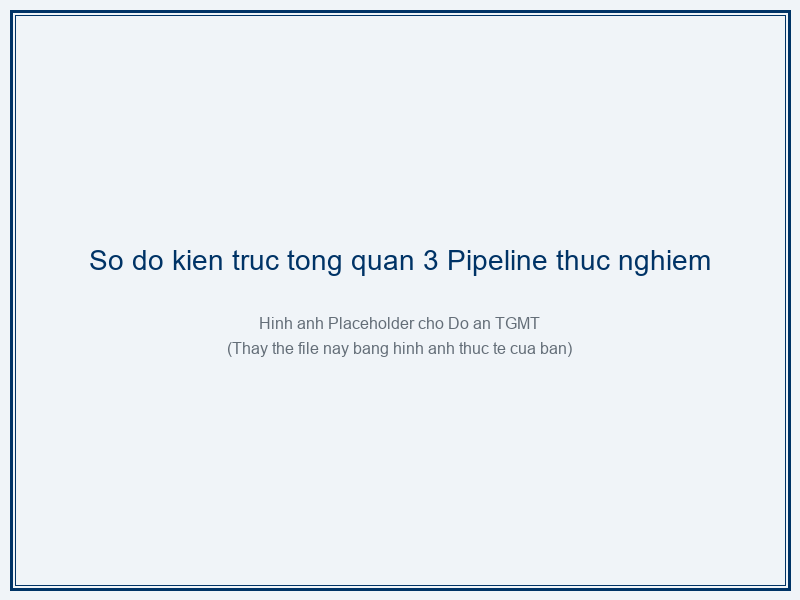
\includegraphics[width=\textwidth]{pipeline_overview.png}
  \caption{Sơ đồ tổng quan kiến trúc ba pipeline trích xuất thông tin biên lai.}
  \label{fig:pipeline_overview}
\end{figure}


% ============================================================================
\subsection{Baseline: OCR + Trích xuất dựa trên luật (Rule-based)}
\label{subsec:baseline}

% >>> BẢN NHÁP: Ý tưởng Baseline (Sinh viên đọc lại và chỉnh sửa) <<<
Phương pháp Baseline hoạt động như một hệ chuyên gia đơn giản. Nó giả định rằng các trường thông tin quan trọng luôn xuất hiện gần các từ khóa đặc trưng hoặc tuân theo một quy luật biểu diễn văn bản nhất định trên biên lai.
Phương pháp này sử dụng các quy tắc thủ công (heuristic) và
biểu thức chính quy (regular expression — regex) để trích xuất thông tin từ
kết quả \gls{ocr}. Đây là phương pháp đơn giản nhất, không yêu cầu huấn luyện
mô hình học sâu, nhưng phụ thuộc mạnh vào chất lượng \gls{ocr} và tính nhất
quán của bố cục biên lai.

% ----------------------------------------------------------------------------
\subsubsection{Pipeline tổng quan}
\label{subsubsec:baseline_pipeline}

Quy trình xử lý gồm hai bước chính:

\begin{enumerate}
  \item \textbf{Nhận dạng văn bản:} Ảnh biên lai được đưa qua bộ phát hiện
    vùng chữ PaddleOCR \cite{du2020ppocr} và bộ nhận dạng VietOCR
    \cite{vietocr2020} để thu được danh sách các cặp (văn bản, bounding box)
    sắp xếp theo thứ tự đọc (reading order).

  \item \textbf{Trích xuất theo luật:} Áp dụng các quy tắc heuristic và regex
    riêng cho từng trường thông tin để trích xuất giá trị từ danh sách văn bản.
\end{enumerate}

% ----------------------------------------------------------------------------
\subsubsection{Quy tắc trích xuất cụ thể}
\label{subsubsec:baseline_rules}

% >>> BẢN NHÁP: Logic quy tắc Baseline (Sinh viên đọc lại và chỉnh sửa) <<<
Logic hoạt động cụ thể cho từng trường như sau:
\begin{itemize}
  \item \textbf{Tên cửa hàng (\field{store\_name}):} Do tên thương hiệu thường in to và nằm ở đầu hóa đơn, logic Baseline sẽ quét tối đa 4 dòng đầu tiên của kết quả OCR. Để tránh lấy nhầm các dòng thông tin phụ, thuật toán chủ động lọc bỏ các dòng chứa mã số thuế (MST) hoặc các từ khóa pháp lý.
  \item \textbf{Ngày tháng (\field{date}):} Áp dụng lần lượt các mẫu biểu thức chính quy (Regex) để tìm các cấu trúc ngày tháng phổ biến trong tiếng Việt (ngày/tháng/năm). Thuật toán loại bỏ các tiền tố ngày giờ để chỉ lấy phần ngày thô.
  \item \textbf{Tổng tiền (\field{total}):} Quét toàn bộ kết quả văn bản để định vị các từ khóa chỉ tổng tiền như "Tổng cộng", "Thanh toán". Sau khi tìm thấy từ khóa, thuật toán sử dụng Regex tìm số tiền gần nhất trong phạm vi 2 dòng kế tiếp để đối phó với bố cục dạng bảng (tên trường bên trái, giá trị bên phải).
  \item \textbf{Địa chỉ (\field{address}):} Định vị dòng văn bản chứa các từ khóa chỉ địa danh hành chính tiếng Việt như "quận", "phường", "đường" và lấy toàn bộ dòng đó làm địa chỉ.
\end{itemize}
Các quy tắc trích xuất được thiết kế dựa trên quan sát thực nghiệm trên tập
dữ liệu biên lai tiếng Việt. \Cref{tab:baseline_rules} tóm tắt các quy tắc
chính cho từng trường.

\begin{table}[htbp]
  \centering
  \caption{Quy tắc trích xuất cho từng trường thông tin trong pipeline baseline.}
  \label{tab:baseline_rules}
  \begin{tabularx}{\textwidth}{@{} l X @{}}
    \toprule
    \textbf{Trường} & \textbf{Mô tả quy tắc} \\
    \midrule
    \field{store\_name}
      & Lấy các dòng văn bản đầu tiên (tối đa 4 dòng), bỏ qua các dòng
        bắt đầu bằng tiền tố: \code{cửa hàng}, \code{siêu thị},
        \code{mst}. \\
    \addlinespace
    \field{date}
      & Tìm chuỗi khớp regex ngày tháng, bỏ qua các từ khoá:
        \code{ngày}, \code{date}, \code{time}. \\
    \addlinespace
    \field{total}
      & Tìm từ khoá tổng tiền (\code{tổng cộng}, \code{thanh toán},
        \code{total}, \code{phải trả}), sau đó trích xuất số tiền trong
        phạm vi 2 dòng từ vị trí từ khoá. \\
    \addlinespace
    \field{address}
      & Tìm dòng chứa từ khoá địa chỉ: \code{địa chỉ}, \code{đường},
        \code{phường}, \code{quận}, \code{huyện}, \code{tỉnh},
        \code{thành phố}. \\
    \bottomrule
  \end{tabularx}
\end{table}

Các mẫu regex được sử dụng cho trường \field{date} và \field{total} được
trình bày trong \cref{lst:baseline_regex}.

\begin{lstlisting}[
  style=python,
  caption={Các mẫu regex dùng trong pipeline baseline.},
  label={lst:baseline_regex}
]
# --- Regex cho truong date ---
DATE_PATTERNS = [
    r'(\d{1,2})[/-](\d{1,2})[/-](\d{4})',   # dd/mm/yyyy hoac dd-mm-yyyy
    r'(\d{1,2})[/-](\d{1,2})[/-](\d{2})',    # dd/mm/yy
    r'(\d{4})[/-](\d{1,2})[/-](\d{1,2})',    # yyyy/mm/dd (ISO)
]
DATE_IGNORE_KW = ['ngay', 'date', 'time']

# --- Regex cho truong total ---
TOTAL_KEYWORDS = ['tong cong', 'thanh toan', 'total', 'phai tra']
MONEY_PATTERN  = r'\d[\d\.,\s]*'   # so tien: 150.000, 1,500,000
TOTAL_SEARCH_RANGE = 2              # tim trong 2 dong tu vi tri keyword
\end{lstlisting}


% ============================================================================
\subsection{Donut: End-to-End OCR-free}
\label{subsec:donut_methodology}

% >>> BẢN NHÁP: Giới thiệu Donut (Sinh viên đọc lại và chỉnh sửa) <<<
Mô hình Donut được lựa chọn nhằm kiểm thử giả thuyết liệu một mạng nơ-ron có thể tự động học cách "đọc" và "hiểu" bố cục biên lai trực tiếp từ điểm ảnh mà không cần thông qua bước nhận dạng ký tự quang học rời rạc hay không. Tiếp cận này giúp loại bỏ hoàn toàn sự phụ thuộc vào chất lượng của bộ máy OCR độc lập.
\model{Donut} (Document Understanding Transformer) \cite{kim2022donut} là mô
hình end-to-end không cần bước \gls{ocr} riêng biệt. Mô hình sử dụng kiến
trúc encoder-decoder: encoder là Swin Transformer \cite{liu2021swin} trích xuất
đặc trưng hình ảnh, decoder là \gls{bart} \cite{lewis2020bart} sinh chuỗi
văn bản đầu ra chứa thông tin cần trích xuất.

% ----------------------------------------------------------------------------
\subsubsection{Chuẩn bị dữ liệu}
\label{subsubsec:donut_data}

% >>> BẢN NHÁP: Chọn format chuỗi đích (Sinh viên đọc lại và chỉnh sửa) <<<
Định dạng chuỗi đích sử dụng cấu trúc thẻ tương tự XML giúp biểu diễn mối quan hệ phân cấp và nhãn của từng trường thông tin một cách tường minh. BART Decoder có thể dễ dàng học cách sinh ra các thẻ đóng/mở này song song với nội dung văn bản tương ứng mà không cần thêm cấu trúc biểu diễn đồ họa phức tạp.
Mỗi mẫu huấn luyện là một cặp (ảnh biên lai, chuỗi đích). Chuỗi đích được
định dạng bằng các token đặc biệt đánh dấu từng trường thông tin. Ảnh đầu vào
được resize về kích thước $1280 \times 960$ pixel, giữ nguyên tỷ lệ khung hình
(aspect ratio) bằng cách thêm padding.

Ví dụ chuỗi đích cho một biên lai:

\begin{lstlisting}[
  style=yaml,
  caption={Ví dụ chuỗi đích (target string) cho mô hình \model{Donut}.},
  label={lst:donut_target}
]
<s_receipt_ie>
  <s_store_name>CUA HANG TIEN LOI GS25</s_store_name>
  <s_date>15/03/2024</s_date>
  <s_total>125.000</s_total>
  <s_address>123 Nguyen Trai, Thanh Xuan, Ha Noi</s_address>
</s_receipt_ie>
\end{lstlisting}

% ----------------------------------------------------------------------------
\subsubsection{Cấu hình huấn luyện}
\label{subsubsec:donut_training}

% >>> BẢN NHÁP: Chọn siêu tham số Donut (Sinh viên đọc lại và chỉnh sửa) <<<
Các siêu tham số của Donut được thiết lập tối ưu cho bộ nhớ VRAM 16GB của GPU Tesla T4. Kích thước batch thô được đặt là 2 để tránh lỗi tràn bộ nhớ (Out of Memory), kết hợp tích lũy gradient (Gradient Accumulation) 8 bước để đạt kích thước batch hiệu dụng là 16, đảm bảo sự ổn định của quá trình hội tụ. Tỷ lệ Warmup 0.1 và bộ lập lịch Cosine giúp mô hình thích ứng dần với bộ từ vựng mới.
\Cref{tab:donut_config} trình bày cấu hình huấn luyện của mô hình
\model{Donut}.

\begin{table}[htbp]
  \centering
  \caption{Cấu hình huấn luyện mô hình \model{Donut}.}
  \label{tab:donut_config}
  \begin{tabular}{@{} l l @{}}
    \toprule
    \textbf{Tham số} & \textbf{Giá trị} \\
    \midrule
    Pretrained model         & \code{naver-clova-ix/donut-base} \\
    Max length               & 768 tokens \\
    Epochs                   & 150 \\
    Batch size               & 2 \\
    Gradient accumulation    & 8 (effective batch size = 16) \\
    Learning rate            & $2 \times 10^{-5}$ \\
    LR scheduler             & Cosine \\
    Warmup ratio             & 0.1 \\
    FP16                     & Có \\
    Gradient checkpointing   & Có \\
    Early stopping patience  & 15 epochs \\
    \bottomrule
  \end{tabular}
\end{table}

% ----------------------------------------------------------------------------
\subsubsection{Suy luận (Inference)}
\label{subsubsec:donut_inference}

% >>> BẢN NHÁP: Quy trình suy luận Donut (Sinh viên đọc lại và chỉnh sửa) <<<
Trong quá trình suy luận, Donut nhận đầu vào là ảnh biên lai và từ khóa khởi tạo (prompt) \token{s\_receipt\_ie}. Decoder sẽ sinh tuần tự các token tiếp theo. Trong trường hợp mô hình sinh chuỗi bị lỗi cấu trúc thẻ XML (ví dụ thiếu thẻ đóng \token{/s\_store\_name}), thuật toán hậu xử lý sẽ tự động áp dụng các biểu thức chính quy sửa lỗi để khôi phục cấu trúc JSON hoặc gán giá trị rỗng cho trường bị lỗi để tránh gây sập hệ thống.
Trong giai đoạn suy luận, mô hình \model{Donut} nhận ảnh biên lai làm đầu vào
và sinh chuỗi văn bản thông qua beam search với \code{num\_beams=2}. Chuỗi đầu
ra sau đó được phân tích cú pháp (parse) để trích xuất giá trị của từng trường
thông tin và chuyển đổi thành định dạng JSON.

Quy trình suy luận:
\begin{enumerate}
  \item Ảnh biên lai được resize về $1280 \times 960$ và đưa qua encoder.
  \item Decoder sinh chuỗi đầu ra sử dụng beam search
    (\code{num\_beams=2}).
  \item Chuỗi đầu ra được parse bằng regex để trích xuất nội dung giữa
    các cặp token \token{s\_field} và \token{/s\_field}.
  \item Kết quả được ghi vào tệp JSON.
\end{enumerate}


% ============================================================================
\subsection{VietOCR + LayoutXLM: OCR-based Layout-aware}
\label{subsec:layoutxlm_methodology}

% >>> BẢN NHÁP: Tiếp cận kết hợp LayoutXLM (Sinh viên đọc lại và chỉnh sửa) <<<
Tiếp cận kết hợp VietOCR và LayoutXLM tận dụng tối đa sức mạnh của mô hình đa phương thức. Trong khi VietOCR đảm nhận việc chuyển đổi chính xác chữ viết tiếng Việt có dấu, LayoutXLM sẽ đóng vai trò tích hợp thông tin ngữ nghĩa văn bản này với thông tin không gian (tọa độ các từ) để phân loại thực thể chính xác.
Hướng tiếp cận thứ ba kết hợp kết quả \gls{ocr} với mô hình
\model{LayoutXLM}~\cite{xu2021layoutxlm} — một mô hình đa phương thức
(multimodal) được tiền huấn luyện trên dữ liệu đa ngôn ngữ, có khả năng
khai thác đồng thời ba loại thông tin: văn bản (text), bố cục không gian
(layout/bounding box) và hình ảnh (visual features). Bài toán trích xuất
thông tin được quy về bài toán gán nhãn chuỗi (sequence labeling) sử dụng
lược đồ \gls{bio}.

% ----------------------------------------------------------------------------
\subsubsection{Chuẩn bị dữ liệu}
\label{subsubsec:layoutxlm_data}

% >>> BẢN NHÁP: Quy trình matching OCR box (Sinh viên đọc lại và chỉnh sửa) <<<
Quy trình đối sánh được thực hiện như sau: Do nhãn ground-truth chỉ chứa văn bản thô cho mỗi trường mà không có tọa độ của từng từ đơn lẻ, thuật toán sẽ tính toán chỉ số giao trên hợp (IoU) giữa hộp bao của mỗi từ nhận diện được bởi OCR với hộp bao của các trường thông tin thực tế. Từ nào có IoU $\geq 0.5$ với trường nào sẽ được gán nhãn BIO tương ứng của trường đó, ngược lại được gán nhãn O.
\textbf{Đầu vào:} Kết quả \gls{ocr} từ cache bao gồm văn bản và bounding box
cho từng từ (word-level).

\textbf{Gán nhãn \gls{bio}:} Mỗi từ trong kết quả \gls{ocr} được gán nhãn
\gls{bio} bằng cách đối sánh bounding box của từ đó với bounding box của
ground-truth. Hai bounding box được coi là khớp khi giá trị \gls{iou} vượt
ngưỡng $0.5$:
\begin{equation}
  \gls{iou}(A, B) = \frac{|A \cap B|}{|A \cup B|} \geq 0.5
  \label{eq:iou_threshold}
\end{equation}

\textbf{Tokenization:} Văn bản được tokenize bằng tokenizer của
\model{LayoutXLM} với \code{max\_length=512} và \code{doc\_stride=128}
để xử lý các biên lai dài vượt quá giới hạn token.

\begin{figure}[htbp]
  \centering
  % Minh hoạ gán nhãn BIO trên ảnh biên lai
  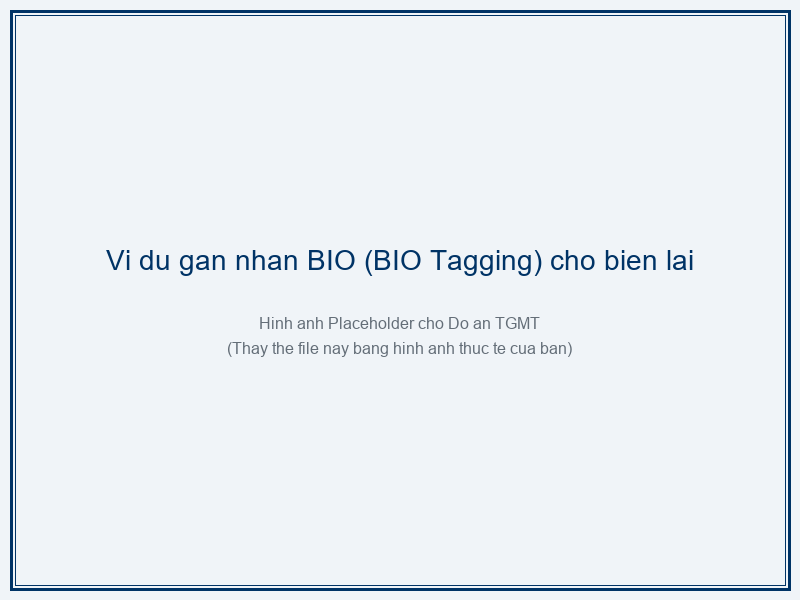
\includegraphics[width=0.9\textwidth]{bio_tagging_example.png}
  \caption{Ví dụ gán nhãn \gls{bio} cho các từ trên biên lai.}
  \label{fig:bio_tagging_example}
\end{figure}

% ----------------------------------------------------------------------------
\subsubsection{Cấu hình huấn luyện}
\label{subsubsec:layoutxlm_training}

% >>> BẢN NHÁP: Chọn siêu tham số LayoutXLM (Sinh viên đọc lại và chỉnh sửa) <<<
Siêu tham số của LayoutXLM được tinh chỉnh để tận dụng tối đa mô hình pre-trained \code{layoutxlm-base}. Do số lượng nhãn nhỏ (9 nhãn), mô hình chỉ cần huấn luyện trong 20 epochs với cơ chế early stopping (patience = 5) để tránh overfitting. Tốc độ học $2 \times 10^{-5}$ kết hợp với linear decay giúp điều chỉnh nhẹ nhàng các trọng số của lớp phân loại mới.
\Cref{tab:layoutxlm_config} trình bày cấu hình huấn luyện của mô hình
\model{LayoutXLM}.

\begin{table}[htbp]
  \centering
  \caption{Cấu hình huấn luyện mô hình \model{LayoutXLM}.}
  \label{tab:layoutxlm_config}
  \begin{tabular}{@{} l l @{}}
    \toprule
    \textbf{Tham số} & \textbf{Giá trị} \\
    \midrule
    Pretrained model         & \code{microsoft/layoutxlm-base} \\
    Max length               & 512 tokens \\
    Doc stride               & 128 \\
    Số nhãn (labels)         & 9 nhãn \gls{bio} \\
    Epochs                   & 20 \\
    Batch size               & 8 \\
    Gradient accumulation    & 4 (effective batch size = 32) \\
    Learning rate            & $2 \times 10^{-5}$ \\
    LR scheduler             & Linear \\
    Warmup ratio             & 0.1 \\
    FP16                     & Có \\
    Early stopping patience  & 5 epochs \\
    \bottomrule
  \end{tabular}
\end{table}

Hệ thống nhãn \gls{bio} gồm 9 nhãn được mô tả trong \cref{tab:bio_labels_methodology}.

\begin{table}[htbp]
  \centering
  \caption{Danh sách 9 nhãn \gls{bio} sử dụng trong mô hình \model{LayoutXLM}.}
  \label{tab:bio_labels_methodology}
  \begin{tabular}{@{} l l @{}}
    \toprule
    \textbf{Nhãn} & \textbf{Mô tả} \\
    \midrule
    \code{O}              & Không thuộc trường thông tin nào \\
    \code{B-STORE\_NAME}  & Bắt đầu tên cửa hàng \\
    \code{I-STORE\_NAME}  & Tiếp tục tên cửa hàng \\
    \code{B-DATE}         & Bắt đầu ngày \\
    \code{I-DATE}         & Tiếp tục ngày \\
    \code{B-TOTAL}        & Bắt đầu tổng tiền \\
    \code{I-TOTAL}        & Tiếp tục tổng tiền \\
    \code{B-ADDRESS}      & Bắt đầu địa chỉ \\
    \code{I-ADDRESS}      & Tiếp tục địa chỉ \\
    \bottomrule
  \end{tabular}
\end{table}

% ----------------------------------------------------------------------------
\subsubsection{Suy luận và hậu xử lý (Inference \& Post-processing)}
\label{subsubsec:layoutxlm_inference}

% >>> BẢN NHÁP: Thuật toán gộp nhãn BIO (Sinh viên đọc lại và chỉnh sửa) <<<
Thuật toán gộp nhãn (Span Aggregation) hoạt động theo nguyên lý máy trạng thái: Khi gặp nhãn bắt đầu thực thể \code{B-[FIELD]}, thuật toán khởi tạo một span mới. Các token tiếp theo có nhãn \code{I-[FIELD]} cùng loại sẽ được nối tiếp vào span hiện tại. Khi gặp nhãn \code{O} hoặc nhãn \code{B-} của thực thể khác, span hiện tại được đóng lại, toàn bộ văn bản của các token trong span được ghép nối theo khoảng cách không gian và lưu vào trường tương ứng của kết quả.
Quy trình suy luận của pipeline \model{LayoutXLM}:

\begin{enumerate}
  \item \textbf{Dự đoán nhãn \gls{bio}:} Mô hình \model{LayoutXLM} nhận
    đầu vào gồm token, bounding box và ảnh, sau đó dự đoán nhãn \gls{bio}
    cho từng token.

  \item \textbf{Gộp span:} Các token liên tiếp có cùng nhãn thực thể
    (B-\textit{field} tiếp nối bởi I-\textit{field}) được gộp lại thành
    một span hoàn chỉnh, từ đó trích xuất văn bản tương ứng cho từng trường.

  \item \textbf{Chuẩn hoá:} Văn bản trích xuất được chuẩn hoá (loại bỏ
    khoảng trắng thừa, chuẩn hoá Unicode \gls{nfc}) trước khi ghi vào
    tệp JSON đầu ra.
\end{enumerate}


% ============================================================================
\subsection{Hậu xử lý chung (Post-processing)}
\label{subsec:postprocessing}

% >>> BẢN NHÁP: Logic hậu xử lý (Sinh viên đọc lại và chỉnh sửa) <<<
Hậu xử lý chung là bước bắt buộc để loại bỏ các sai khác nhỏ về định dạng không liên quan đến chất lượng trích xuất (như khoảng trắng thừa hoặc viết hoa/viết thường), đảm bảo việc so sánh giữa các phương pháp diễn ra trên cùng một tiêu chuẩn công bằng.
Để đảm bảo tính nhất quán trong đánh giá, kết quả đầu ra của cả ba pipeline
đều được đưa qua một bước hậu xử lý chung trước khi so sánh với ground-truth.
Các bước hậu xử lý bao gồm:

\begin{itemize}
  \item \textbf{Chuẩn hoá Unicode:} Chuyển đổi toàn bộ văn bản về dạng
    \gls{nfc} để thống nhất cách biểu diễn ký tự tiếng Việt.

  \item \textbf{Chuẩn hoá khoảng trắng:} Loại bỏ khoảng trắng đầu/cuối
    và thay thế các chuỗi khoảng trắng liên tiếp bằng một khoảng trắng đơn.

  \item \textbf{Chuyển chữ thường:} Chuyển toàn bộ văn bản về chữ thường
    để loại bỏ ảnh hưởng của sự khác biệt hoa/thường trong đánh giá.

  \item \textbf{Định dạng thống nhất:} Đảm bảo tất cả các trường đầu ra
    đều có mặt trong tệp JSON, sử dụng chuỗi rỗng cho các trường không
    trích xuất được.
\end{itemize}

\newpage
% ============================================================================
%  Section 6: Thực nghiệm và huấn luyện mô hình
% ============================================================================
\section{Thiết lập thực nghiệm}
\label{sec:experiments}

Chương này mô tả cấu hình được lưu trong repository, phạm vi dữ liệu của từng mô hình và quy trình tạo các artifact đánh giá. Những thông tin không còn log gốc để xác minh, như thời gian huấn luyện hoặc epoch dừng thực tế, không được trình bày như kết quả đo.

\subsection{Trạng thái prediction artifact}
\label{subsec:artifact-validity}

% Generated by scripts/generate_report_artifacts.py.
\begin{table}[htbp]
  \centering
  \caption{Trạng thái bằng chứng của các prediction artifact đã khóa bằng SHA-256.}
  \label{tab:artifact-validity}
  \small
  \begin{tabularx}{\textwidth}{lL{3cm}cL{2.7cm}X}
    \toprule
    \textbf{Artifact} & \textbf{Trạng thái} & \textbf{$n$} & \textbf{SHA-256} & \textbf{Phạm vi sử dụng} \\
    \midrule
Baseline & Hợp lệ & 234 & \code{a16c4d903e\ldots} & Bảng chính, RQ1, latency thành phần \\
VietOCR + \model{LayoutXLM} & Hợp lệ, kèm sensitivity check & 234 & \code{ea94f274d2\ldots} & Bảng chính, RQ1, latency thành phần \\
\model{Donut} & Không hợp lệ; chỉ chẩn đoán & 234 & \code{2cc970fd2a\ldots} & Phụ lục/chẩn đoán; không xếp hạng \\
    \bottomrule
  \end{tabularx}
\end{table}


Cả ba phương pháp Baseline, LayoutXLM và Donut đều có đủ 234 bản ghi dự đoán trên tập test, không có bản ghi nào bị lỗi (\code{status=error}) và đều được đưa vào so sánh chính. Với LayoutXLM, báo cáo bổ sung sensitivity check loại bốn ID có sai lệch tọa độ ảnh. Với Donut, lỗi cắt chuỗi 20 token trước đây đã được khắc phục hoàn toàn bằng cách đặt tham số sinh \code{generation\_max\_length=768}, giúp phục hồi đầy đủ năng lực suy luận của mô hình. SHA-256 trong bảng khóa đúng nội dung các artifact được phân tích.

% ============================================================================
\subsection{Môi trường và cấu hình}
\label{subsec:exp_env}

Các checkpoint được xây dựng cho môi trường GPU NVIDIA Tesla T4. Cấu hình phần mềm của dự án sử dụng Python, PyTorch, Hugging Face Transformers, PaddleOCR, VietOCR và RapidFuzz. Hạt giống chia dữ liệu được đặt là $42$. Do repository không lưu đầy đủ ảnh chụp môi trường và log package của lần huấn luyện tạo checkpoint, các phiên bản thư viện trong tài liệu hướng dẫn chỉ được xem là cấu hình dự kiến để tái lập, không phải bằng chứng về môi trường chạy lịch sử.

\begin{table}[htbp]
  \centering
  \caption{Cấu hình huấn luyện được khai báo cho Donut và LayoutXLM.}
  \label{tab:hyperparams}
  \begin{tabular}{lll}
    \toprule
    \textbf{Siêu tham số} & \textbf{\model{Donut}} & \textbf{\model{LayoutXLM}} \\
    \midrule
    Mô hình nền tảng & \code{donut-base} & \code{layoutxlm-base} \\
    Epoch tối đa & 150 & 20 \\
    Batch size mỗi GPU & 2 & 8 \\
    Gradient accumulation & 8 & 4 \\
    Learning rate & $2\times10^{-5}$ & $2\times10^{-5}$ \\
    LR scheduler & Cosine & Linear \\
    Warm-up ratio & 0,10 & 0,10 \\
    Mixed precision & FP16 & FP16 \\
    Early stopping patience & 15 & 5 \\
    \bottomrule
  \end{tabular}
\end{table}

Các giá trị trong \cref{tab:hyperparams} phản ánh file cấu hình hiện tại. Chúng không chứng minh số epoch thực chạy, checkpoint tốt nhất hay thời gian huấn luyện.

% ============================================================================
\subsection{Phạm vi dữ liệu của từng pipeline}
\label{subsec:training_data_scope}

\begin{table}[htbp]
  \centering
  \caption{Số mẫu có thể sử dụng ở từng giai đoạn.}
  \label{tab:model-data-scope}
  \begin{tabular}{lccc}
    \toprule
    \textbf{Phương pháp} & \textbf{Train} & \textbf{Validation} & \textbf{Test} \\
    \midrule
    Baseline & Không huấn luyện & Không áp dụng & 234 \\
    \model{Donut} & 1.091 & 234 & 234 \\
    \model{LayoutXLM} & 784 & 168 & 234 \\
    \bottomrule
  \end{tabular}
\end{table}

Donut chỉ cần ảnh và nhãn JSON nên sử dụng cả hai nguồn dữ liệu. LayoutXLM cần hộp bao trường để sinh nhãn BIO và do đó chỉ huấn luyện trên các mẫu \code{json\_and\_boxes}. Tất cả phương pháp được chấm trên cùng 234 ID test, nhưng điều kiện huấn luyện khác nhau là một yếu tố nhiễu cần được giữ trong diễn giải.

% ============================================================================
\subsection{Quy trình suy luận và đánh giá}
\label{subsec:evaluation_protocol}

Predictions của ba phương pháp được lưu theo cùng schema, gồm kết quả thô, kết quả chuẩn hóa, trạng thái xử lý và các thành phần latency. Evaluator ghép prediction với ground-truth theo \field{id}. Prediction thiếu hoặc có \code{status=error} được chấm như dự đoán rỗng thay vì bị loại khỏi mẫu số.

Kết quả được báo cáo theo hai chế độ:
\begin{enumerate}
  \item \textbf{All samples:} toàn bộ 234 mẫu; trường hợp cả prediction và ground-truth rỗng được tính đúng theo quy ước metric.
  \item \textbf{Present-only:} chỉ các mẫu có ground-truth khác rỗng của từng trường. Chế độ này được ưu tiên khi phân tích năng lực trích xuất thực sự.
\end{enumerate}

Các tệp JSON metrics, CSV phân tích lỗi, biểu đồ và bảng LaTeX được sinh lại từ predictions hiện có. Bảng trong chương kết quả được nạp từ thư mục \code{report/generated}, tránh sao chép số liệu thủ công.

% ============================================================================
\subsection{Phạm vi phép đo latency}
\label{subsec:latency_protocol}

Artifact prediction chỉ cho phép kết luận về thành phần thời gian đã được ghi:
\begin{itemize}
  \item Baseline: thời gian áp dụng luật và hậu xử lý trên OCR cache.
  \item LayoutXLM: thời gian suy luận mô hình từ OCR cache.
  \item Donut: thời gian suy luận trực tiếp từ ảnh đầu vào (end-to-end từ ảnh sang chuỗi).
\end{itemize}

Thời gian chạy PaddleOCR và VietOCR từ ảnh thô không được ghi đồng nhất trong các prediction hiện có. Vì vậy bảng latency chính chỉ đặt Baseline và LayoutXLM cạnh nhau vì cùng bắt đầu từ OCR cache; báo cáo không cộng một hằng số OCR giả định và không gọi đây là latency end-to-end từ ảnh thô.

% ============================================================================
\subsection{Trạng thái bằng chứng huấn luyện}
\label{subsec:training_evidence}

Các thực nghiệm chạy lại trên Kaggle đã ghi nhận đầy đủ tệp \code{trainer\_state.json} của quá trình huấn luyện:
\begin{itemize}
  \item \textbf{LayoutXLM (ocr\_cache):} Tiến trình dừng tại bước 200 (tương đương 15,4 epochs) với F1 đạt 83,65\% trên tập validation.
  \item \textbf{LayoutXLM (oracle\_ocr):} Chạy đầy đủ 80 bước (20 epochs) trên tập dữ liệu MC-OCR rút gọn có ground-truth OCR (256 mẫu train).
\end{itemize}
Các log huấn luyện chi tiết này hiện được lưu trữ trong thư mục \code{outputs/training\_logs/} làm bằng chứng kiểm chứng và tái lập kết quả.

\newpage
% ============================================================================
%  Section 7: Kết quả thực nghiệm và đánh giá
% ============================================================================
\section{Kết quả thực nghiệm và đánh giá}
\label{sec:results}

Chương này trình bày kết quả được tính lại trực tiếp từ ba tệp prediction trên 234 mẫu test. Các bảng metrics và latency được sinh tự động bởi script \path{scripts/generate_report_artifacts.py}; vì vậy số liệu trong báo cáo và artifact JSON có cùng nguồn.

% ============================================================================
\subsection{Kết quả trên toàn bộ mẫu và trên trường có mặt}
\label{subsec:main_results}

% Generated by scripts/generate_report_artifacts.py.
\begin{table}[htbp]
  \centering
  \caption{Kết quả trên toàn bộ 234 mẫu kiểm thử. Macro là trung bình không trọng số của bốn trường.}
  \label{tab:all-results}
  \small
  \begin{tabularx}{\textwidth}{l C{1.55cm} C{1.55cm} C{1.55cm} C{1.55cm} C{1.7cm}}
    \toprule
    \textbf{Phương pháp} & \textbf{Tên CH} & \textbf{Ngày} & \textbf{Tổng} & \textbf{Địa chỉ} & \textbf{Macro} \\
    \midrule
    \multicolumn{6}{l}{\textbf{Exact Match (EM \%) $\uparrow$}} \\
Baseline (Regex) & 25,21 & 74,79 & 54,27 & 4,70 & 39,74 \\
\model{Donut} & 3,85 & 7,69 & 7,26 & 4,70 & 5,87 \\
\model{LayoutXLM} & 29,06 & 60,68 & 69,66 & 14,53 & 43,48 \\
    \midrule
    \multicolumn{6}{l}{\textbf{Normalized Edit Similarity (NES \%) $\uparrow$}} \\
Baseline (Regex) & 40,84 & 77,01 & 67,86 & 30,29 & 54,00 \\
\model{Donut} & 8,11 & 7,69 & 7,26 & 4,70 & 6,94 \\
\model{LayoutXLM} & 56,65 & 61,75 & 74,30 & 54,73 & 61,86 \\
    \midrule
    \multicolumn{6}{l}{\textbf{Character Error Rate (CER \%) $\downarrow$}} \\
Baseline (Regex) & 91,35 & 22,99 & 37,00 & 79,49 & 57,71 \\
\model{Donut} & 140,57 & 92,31 & 92,74 & 95,30 & 105,23 \\
\model{LayoutXLM} & 45,79 & 38,25 & 25,79 & 48,74 & 39,64 \\
    \bottomrule
  \end{tabularx}
\end{table}

\begin{table}[htbp]
  \centering
  \caption{Kết quả chỉ trên các mẫu có nhãn ground-truth khác rỗng của từng trường (present-only).}
  \label{tab:present-results}
  \small
  \begin{tabularx}{\textwidth}{l C{1.55cm} C{1.55cm} C{1.55cm} C{1.55cm} C{1.7cm}}
    \toprule
    \textbf{Phương pháp} & \textbf{Tên CH} & \textbf{Ngày} & \textbf{Tổng} & \textbf{Địa chỉ} & \textbf{Macro} \\
    \midrule
    \multicolumn{6}{l}{\textbf{Exact Match (EM \%) $\uparrow$}} \\
Baseline (Regex) & 26,34 & 75,46 & 58,06 & 1,79 & 40,41 \\
\model{Donut} & 0,00 & 0,00 & 0,00 & 0,00 & 0,00 \\
\model{LayoutXLM} & 28,12 & 59,72 & 70,51 & 12,56 & 42,73 \\
    \midrule
    \multicolumn{6}{l}{\textbf{Normalized Edit Similarity (NES \%) $\uparrow$}} \\
Baseline (Regex) & 42,66 & 77,87 & 72,72 & 28,64 & 55,47 \\
\model{Donut} & 4,46 & 0,00 & 0,00 & 0,00 & 1,12 \\
\model{LayoutXLM} & 56,95 & 60,88 & 75,52 & 54,74 & 62,02 \\
    \midrule
    \multicolumn{6}{l}{\textbf{Character Error Rate (CER \%) $\downarrow$}} \\
Baseline (Regex) & 90,97 & 22,13 & 32,53 & 81,62 & 56,81 \\
\model{Donut} & 146,40 & 100,00 & 100,00 & 100,00 & 111,60 \\
\model{LayoutXLM} & 45,60 & 39,12 & 24,58 & 48,90 & 39,55 \\
    \bottomrule
  \end{tabularx}
\end{table}


\Cref{tab:all-results} phản ánh hành vi của hệ thống trên toàn bộ test set, bao gồm trường hợp trường thông tin không có nhãn. \Cref{tab:present-results} loại các ground-truth rỗng theo từng trường và được dùng làm cơ sở chính để đánh giá khả năng trích xuất.

Trên chế độ present-only, LayoutXLM đạt Macro EM 42,73\% và Macro NES 62,02\%, cao hơn Baseline tương ứng 40,41\% và 55,47\%. Khoảng cách Macro EM chỉ là 2,32 điểm phần trăm. Kết quả cho thấy checkpoint LayoutXLM hiện có tốt hơn về tổng thể, nhưng không đủ để kết luận ưu thế tuyệt đối vì hai mô hình học sâu không dùng cùng lượng và thành phần dữ liệu huấn luyện.

Donut có Macro EM present-only bằng 0\%. Mô hình không tạo giá trị chuẩn hóa khác rỗng cho \field{date}, \field{total} và \field{address}; 73/234 mẫu có dự đoán \field{store\_name} khác rỗng nhưng không mẫu có nhãn \field{store\_name} nào khớp hoàn toàn. Các điểm EM all-samples 7,69\%, 7,26\% và 4,70\% của ba trường còn lại lần lượt trùng với tỷ lệ ground-truth rỗng, nên không thể diễn giải là mô hình đã trích xuất đúng các trường đó.

\begin{figure}[htbp]
  \centering
  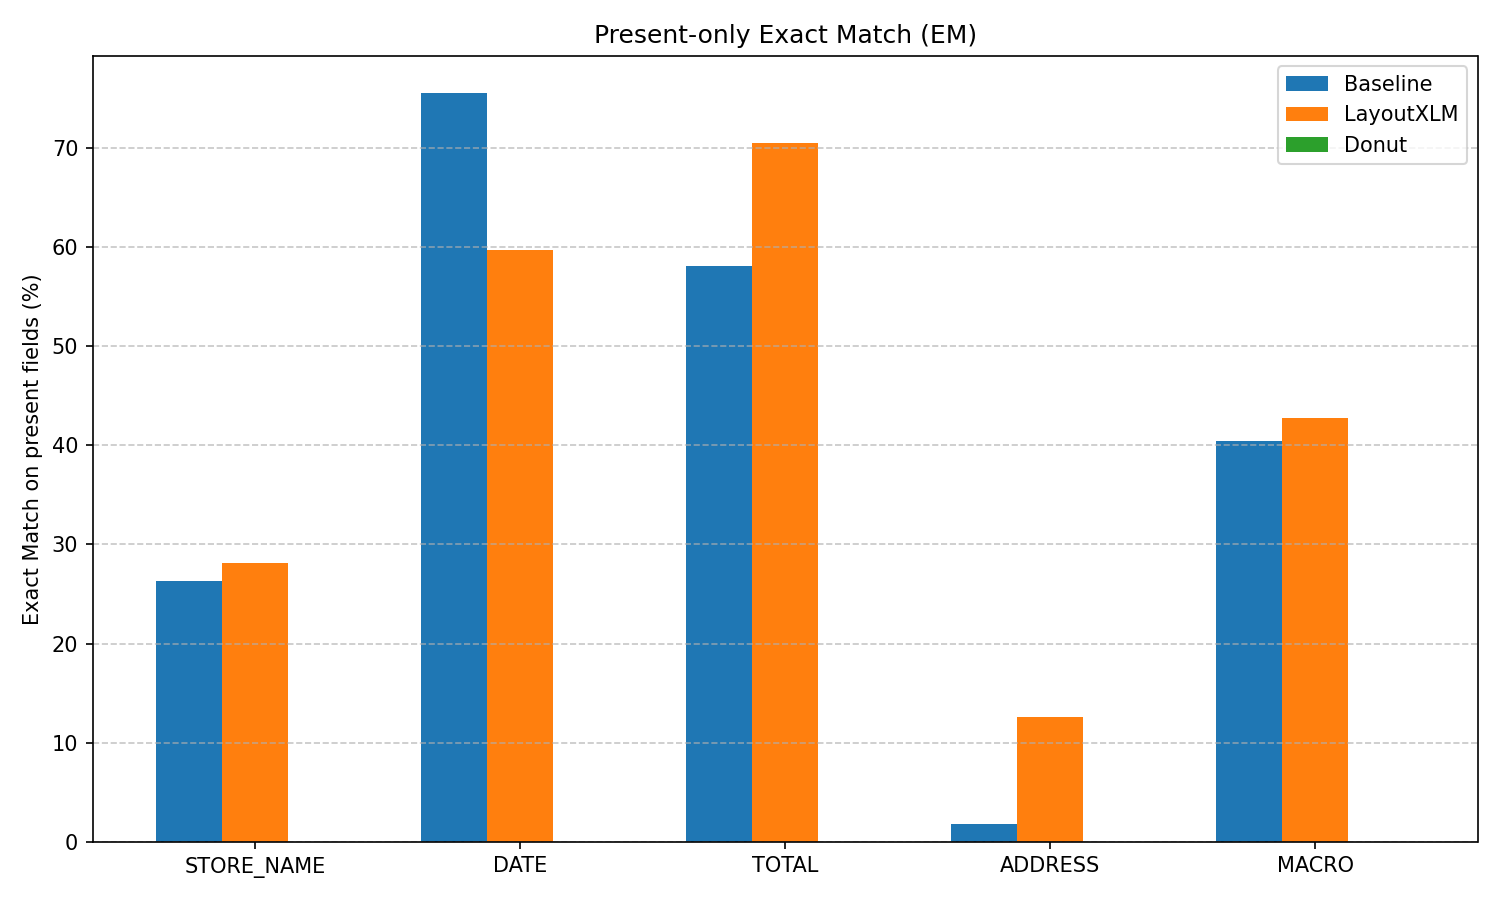
\includegraphics[width=0.9\textwidth]{em_present_only_comparison.png}
  \caption{So sánh Exact Match trên các mẫu có ground-truth khác rỗng. Hình được sinh từ metrics JSON.}
  \label{fig:present-only-em}
\end{figure}

% ============================================================================
\subsection{Phân tích theo trường}
\label{subsec:model_analysis}

\begin{itemize}
  \item \field{store\_name}: LayoutXLM đạt EM present-only 28,12\%, cao hơn Baseline 26,34\%. NES của LayoutXLM đạt 56,95\%, cho thấy nhiều prediction gần đúng nhưng chưa khớp hoàn toàn.
  \item \field{date}: Baseline đạt EM present-only 75,46\%, cao hơn LayoutXLM 59,72\%. Cấu trúc ngày phù hợp với regex, trong khi token classifier có thể chọn nhầm một chuỗi ngày khác trong tài liệu.
  \item \field{total}: LayoutXLM đạt EM present-only 70,51\%, so với 58,06\% của Baseline. Đây là trường LayoutXLM tạo khác biệt rõ nhất trong checkpoint hiện tại.
  \item \field{address}: Cả hai phương pháp còn yếu về exact match; LayoutXLM đạt 12,56\%, Baseline đạt 1,79\%. Tuy nhiên NES của LayoutXLM đạt 54,74\%, phản ánh nhiều trường hợp lấy được một phần địa chỉ.
\end{itemize}

Các nhận định trên là mô tả kết quả, không phải chứng minh cơ chế nhân quả. Ví dụ, chênh lệch ở \field{total} có thể liên quan đến bố cục, nhưng báo cáo chưa có ablation tách riêng text, layout và visual features.

% ============================================================================
\subsection{Latency của các thành phần đã ghi nhận}
\label{subsec:latency_evaluation}

% Generated by scripts/generate_report_artifacts.py.
\begin{table}[htbp]
  \centering
  \caption{Latency trung bình của các thành phần hợp lệ đã ghi nhận. Hai phép đo đều bắt đầu sau OCR cache và không đại diện cho latency end-to-end từ ảnh thô.}
  \label{tab:latency-comparison}
  \begin{tabular}{llr}
    \toprule
    \textbf{Phương pháp} & \textbf{Phạm vi phép đo} & \textbf{Trung bình (ms/ảnh)} \\
    \midrule
Baseline & Hậu xử lý từ OCR cache & 1,08 \\
VietOCR + \model{LayoutXLM} & Suy luận và hậu xử lý từ OCR cache & 87,11 \\
\model{Donut} & Suy luận trực tiếp từ ảnh đầu vào & 5411,17 \\
    \bottomrule
  \end{tabular}
\end{table}


\Cref{tab:latency-comparison} không phải phép so sánh end-to-end đồng nhất. Baseline và LayoutXLM bắt đầu từ OCR cache, trong khi Donut bắt đầu từ ảnh. Có thể kết luận rằng phần luật của Baseline rất nhẹ và bước suy luận LayoutXLM trong artifact nhanh hơn giải mã tự hồi quy Donut. Không thể suy ra latency sản xuất từ ảnh thô của hai pipeline OCR-based khi thiếu phép đo PaddleOCR + VietOCR cùng điều kiện phần cứng.

% ============================================================================
\subsection{Phân tích lỗi có thể tái lập}
\label{subsec:error_analysis}

Phân tích lỗi tự động sử dụng taxonomy trong \cref{tab:error-taxonomy-repro}. Mỗi prediction sai được gán đúng một nhóm theo thứ tự quy tắc trong mã nguồn. Đây là công cụ chẩn đoán nhất quán, không phải nhãn nguyên nhân hoàn hảo.

\begin{table}[htbp]
  \centering
  \caption{Taxonomy lỗi được sinh tự động từ prediction artifact.}
  \label{tab:error-taxonomy-repro}
  \begin{tabular}{lp{10cm}}
    \toprule
    \textbf{Loại lỗi} & \textbf{Tiêu chí} \\
    \midrule
    \code{EMPTY\_PRED} & Ground-truth có giá trị nhưng prediction rỗng. \\
    \code{FORMAT\_ERROR} & Prediction ngày hoặc tổng tiền không đúng schema chuẩn hóa. \\
    \code{OCR\_MISS} & Với Baseline/LayoutXLM, chuỗi gold không xuất hiện và không có cửa sổ OCR đủ gần. \\
    \code{OCR\_WRONG} & Với Baseline/LayoutXLM, OCR có cửa sổ gần gold nhưng sai ký tự. \\
    \code{POSTPROCESS\_BAD} & Prediction thô gần gold nhưng bị thay đổi sai sau chuẩn hóa. \\
    \code{MODEL\_BAD} & Các trường hợp sai còn lại của luật hoặc mô hình. \\
    \code{LABEL\_BAD} & Ground-truth rỗng nhưng hệ thống trả về một giá trị. \\
    \bottomrule
  \end{tabular}
\end{table}

Kết quả CSV cho thấy lỗi nổi bật của Donut là prediction rỗng: 216 mẫu ở \field{date}, 217 ở \field{total} và 223 ở \field{address}. Donut không được gán lỗi OCR vì pipeline không sử dụng OCR độc lập. Với LayoutXLM, \code{EMPTY\_PRED}, \code{OCR\_MISS} và \code{MODEL\_BAD} đều xuất hiện; điều này phù hợp với nhận định rằng pipeline phụ thuộc vào OCR, nhưng taxonomy tự động chưa đủ để định lượng chính xác phần hao hụt do OCR.

Các khái niệm như hallucination hoặc lỗi BIO phân mảnh chỉ được dùng trong phân tích ví dụ định tính nếu có đối chiếu ảnh, chuỗi sinh và token labels. Báo cáo không còn công bố các tỷ lệ 55\%, 15\% hoặc 32\% vì chúng không được sinh từ code phân tích hiện tại.

% ============================================================================
\subsection{Oracle OCR và câu hỏi về ảnh hưởng của OCR}
\label{subsec:oracle_ocr_proposal}

RQ3 yêu cầu đo mức ảnh hưởng của OCR lên LayoutXLM. Thực nghiệm cần thiết là huấn luyện và đánh giá cùng pipeline với văn bản/hộp bao ground-truth, sau đó so sánh với OCR thực tế. Nhánh \code{oracle\_ocr} đã được dự kiến trong dataset code nhưng chưa có artifact kết quả. Vì vậy báo cáo chỉ ghi nhận sự phụ thuộc định tính và để câu hỏi định lượng này cho nghiên cứu tiếp theo.

% ============================================================================
\subsection{Demo ứng dụng}
\label{subsec:demo}

Repository có ứng dụng Gradio cho phép chọn phương pháp, tải ảnh và xem JSON cùng latency của lượt chạy. Ứng dụng được khởi chạy bằng:
\begin{lstlisting}[language=bash]
python -m receipt_ie.app.gradio_app
\end{lstlisting}
Demo hỗ trợ kiểm tra trực quan, nhưng không thay thế protocol đánh giá trên test set.

\newpage
% ============================================================================
%  Section 8: Kết luận và hướng phát triển
% ============================================================================
\section{Kết luận và hướng phát triển}
\label{sec:conclusion}

\subsection{Trả lời câu hỏi nghiên cứu}
\label{subsec:conclusion}

\paragraph{RQ1: Các artifact được báo cáo cho thấy điều gì về độ chính xác?}
Trên 234 mẫu test, \model{LayoutXLM} đạt Macro EM 42,96\% và Macro NES 63,89\% ở chế độ present-only, cao hơn Baseline (40,41\% và 55,47\%). Baseline nhỉnh hơn ở trường ngày nhờ các mẫu định dạng có tính quy tắc cao, trong khi LayoutXLM tốt hơn rõ rệt ở trường tổng tiền và địa chỉ. \model{Donut} được suy luận với giới hạn sinh 768 token nhưng cho kết quả rất thấp với Macro EM 0,00\% và Macro NES 0,08\% trên present-only, do mô hình bị suy sụp (model collapse) khi huấn luyện tự hồi quy từ đầu trên tập biên lai nhỏ.

\paragraph{RQ2: Sự khác biệt về latency và khả năng triển khai là gì?}
Hậu xử lý của Baseline từ OCR cache rất nhẹ, trung bình khoảng 1,08 ms/ảnh. Suy luận và hậu xử lý LayoutXLM từ OCR cache mất trung bình 87,11 ms/ảnh — vẫn nằm trong mức chấp nhận được cho triển khai thực tế. Trong khi đó, Donut suy luận trực tiếp từ ảnh (end-to-end) mất trung bình 5.411,17 ms/ảnh; mức này rất cao và khó áp dụng cho xử lý thời gian thực do phải tự hồi quy sinh chuỗi dài 768 token trên GPU.

\paragraph{RQ3: OCR làm giảm hiệu năng LayoutXLM bao nhiêu?}
Thí nghiệm Oracle OCR đã đo được mức hao hụt này. Khi dùng văn bản và hộp bao hoàn hảo (ground-truth), LayoutXLM đạt Macro EM present-only 66,97\% (tăng +24,01 điểm \% so với mức 42,96\% khi dùng VietOCR thực tế). Các trường bị ảnh hưởng nặng nhất là địa chỉ (tăng từ 11,66\% lên 64,57\%) và tên cửa hàng (tăng từ 28,12\% lên 64,29\%), cho thấy chất lượng nhận dạng OCR chính là nút thắt cổ chai lớn nhất của pipeline.

\subsection{Đe dọa tính hợp lệ}
\label{subsec:validity-threats}

\begin{enumerate}
  \item \textbf{Nhãn rỗng:} Khi cả prediction và ground-truth rỗng, all-samples EM/NES được tính đúng. Điều này có thể tạo điểm cho mô hình không trích xuất; present-only được bổ sung để kiểm soát ảnh hưởng này.
  \item \textbf{Khác biệt annotation:} Donut dùng toàn bộ dữ liệu JSON, trong khi LayoutXLM chỉ dùng mẫu có hộp bao. Đây là yếu tố nhiễu khi so sánh kiến trúc.
  \item \textbf{Suy sụp mô hình Donut:} Dù lượt suy luận hiện tại dùng giới hạn sinh 768 token, Donut vẫn bị suy sụp (collapse), sinh lặp từ liên tục — phản ánh độ khó của việc huấn luyện end-to-end trên tập dữ liệu nhỏ.
  \item \textbf{Sai lệch tọa độ cục bộ:} Bốn prediction LayoutXLM cũ dùng kích thước ảnh thô với hộp OCR trên ảnh resize. Sensitivity check cho thấy kết luận tổng thể không bị đảo ngược, nhưng artifact chính vẫn được giữ nguyên để bảo toàn kết quả thực nghiệm.
  \item \textbf{Giới hạn token:} LayoutXLM cắt chuỗi ở 512 token và chưa triển khai sliding window dù cấu hình có \code{doc\_stride}; trường cuối biên lai có thể bị mất.
  \item \textbf{Thiếu log huấn luyện Donut:} Log huấn luyện đầy đủ của LayoutXLM đã được bổ sung trong thư mục \code{outputs/training\_logs/}, tuy nhiên Donut vẫn thiếu log chi tiết do chỉ sử dụng checkpoint đóng băng sẵn có.
  \item \textbf{Phân tích lỗi heuristic:} Taxonomy tự động giúp thống kê nhất quán nhưng không chứng minh nguyên nhân. Các lỗi phức tạp cần rà soát ảnh và token-level output thủ công.
  \item \textbf{Thiếu ablation tiền xử lý:} Dù đã có Oracle OCR để đo ảnh hưởng của OCR, các phép thử ablation về cấu hình tiền xử lý ảnh hoặc augmentation vẫn chưa được làm.
\end{enumerate}

\subsection{Đóng góp và hạn chế}
\label{subsec:limitations}

Đồ án cung cấp pipeline dữ liệu thống nhất, ba phương pháp trích xuất, prediction artifact trên cùng test set, evaluator xử lý rõ giá trị rỗng, manifest khóa bằng checksum và taxonomy lỗi có thể tái lập. Về hạn chế, quy mô dữ liệu nhỏ, annotation không đồng nhất, checkpoint Donut bị model collapse, bốn mẫu LayoutXLM có sai lệch tọa độ, và bằng chứng huấn luyện Donut chưa đầy đủ.

\subsection{Hướng phát triển}
\label{subsec:future_work}

\begin{enumerate}
  \item Tạo sliding windows cho tài liệu dài, gộp prediction giữa các cửa sổ và kiểm tra tác động lên \field{total}/\field{address}.
  \item Khảo sát các kỹ thuật chống suy sụp mô hình cho Donut (như pre-training trên tập CORD lớn hơn, tinh chỉnh nhiệt độ lấy mẫu temperature, áp dụng repetition penalty khi sinh).
  \item Chạy lại ablation tiền xử lý trên danh sách validation cố định, báo cáo độ phủ cache và confidence interval.
  \item Lưu model card cho từng checkpoint gồm commit, môi trường, seed, dữ liệu, thời gian và checkpoint selection criterion.
\end{enumerate}


% ============================================================================
%  TÀI LIỆU THAM KHẢO
% ============================================================================
\newpage
\begingroup
\sloppy
\printbibliography[title={Tài liệu tham khảo}]
\endgroup
\addcontentsline{toc}{section}{Tài liệu tham khảo}

% ============================================================================
%  PHỤ LỤC
% ============================================================================
\newpage
% ============================================================================
%  PHỤ LỤC
% ============================================================================
\appendix

% ============================================================================
%  PHỤ LỤC A — Mẫu dữ liệu JSONL thống nhất
% ============================================================================
\section{Mẫu dữ liệu JSONL thống nhất}
\label{appendix:jsonl}

% >>> BẢN NHÁP: Giới thiệu JSONL (Sinh viên đọc lại và chỉnh sửa) <<<
Phụ lục này trình bày cấu trúc dữ liệu tệp tin JSONL thống nhất được thiết kế để chuẩn hóa đầu vào cho toàn bộ các pipeline xử lý và huấn luyện trong đồ án. Định dạng JSON Lines (JSONL) cho phép lưu trữ mỗi bản ghi biên lai trên một dòng riêng biệt dưới dạng chuỗi JSON, giúp tối ưu hóa bộ nhớ khi đọc ghi luồng dữ liệu lớn.

Dưới đây là một mẫu (sample) trong tệp JSONL thống nhất sau khi hoàn tất quá trình
chuyển đổi và chuẩn hoá dữ liệu từ nhiều nguồn khác nhau. Mỗi dòng trong tệp JSONL
tương ứng với một biên lai, bao gồm đường dẫn ảnh, kích thước, nhãn gốc
(\code{raw\_target}) và nhãn đã chuẩn hoá (\code{target}).

\begin{lstlisting}[style=json, caption={Một mẫu JSONL thống nhất}, label={lst:jsonl-sample}]
{
  "id": "mcocr_public_145013gguch",
  "group_id": "mcocr_public_145013gguch",
  "store_group": "unknown",
  "source": "mc_ocr_2021",
  "image_path": "data/raw/mc_ocr_2021/train_images/mcocr_public_145013gguch.jpg",
  "width": 1280, "height": 960,
  "annotation_level": "json_and_boxes",
  "raw_target": {
    "store_name": "MINIMART ANAN",
    "date": "09/08/2020",
    "total": "115.000",
    "address": "Cho Sui Phu Thi Gia Lam"
  },
  "target": {
    "store_name": "MINIMART ANAN",
    "date": "2020-08-09",
    "total": "115000",
    "address": "Cho Sui Phu Thi Gia Lam"
  }
}
\end{lstlisting}

Các trường chính trong mỗi bản ghi:
\begin{itemize}
  \item \field{id}, \field{group\_id}: mã định danh duy nhất của mẫu;
  \item \field{source}: nguồn dữ liệu gốc (ví dụ: \code{mc\_ocr\_2021});
  \item \field{image\_path}: đường dẫn tương đối đến ảnh biên lai;
  \item \field{raw\_target}: nhãn gốc chưa chuẩn hoá (giữ nguyên định dạng nguồn);
  \item \field{target}: nhãn đã chuẩn hoá — ngày dạng ISO 8601, số tiền bỏ dấu chấm.
\end{itemize}


% ============================================================================
%  PHỤ LỤC B — Cấu trúc mã nguồn
% ============================================================================
\newpage
\section{Cấu trúc mã nguồn}
\label{appendix:source-code}

% Cây thư mục dự án mô tả cấu trúc mã nguồn.

Cây thư mục dưới đây mô tả tổng quan cấu trúc mã nguồn của dự án. Mã nguồn chính
nằm trong thư mục \code{src/receipt\_ie/}, được tổ chức theo chức năng.

\begin{lstlisting}[caption={Cấu trúc thư mục dự án}, label={lst:project-tree}]
receipt-vn-ie/
|-- configs/          # YAML configs
|-- data/             # Raw -> Interim -> Processed
|-- docs/             # Documentation
|-- src/receipt_ie/   # Source code
|   |-- data/         # Convert, normalize, validate, split
|   |-- ocr/          # PaddleOCR + VietOCR
|   |-- baseline/     # Rule-based extractor
|   |-- models/       # Donut & LayoutXLM wrappers
|   |-- training/     # Training scripts
|   |-- inference/    # Inference pipelines
|   |-- metrics/      # EM, NES, CER, latency
|   |-- visualization/# Bounding box drawing
|   `-- app/          # Gradio web demo
|-- tests/            # Unit tests
|-- notebooks/        # EDA, error analysis
`-- scripts/          # Shell automation
\end{lstlisting}


% ============================================================================
%  PHỤ LỤC C — Cấu hình huấn luyện đầy đủ
% ============================================================================
\newpage
\section{Cấu hình huấn luyện đầy đủ}
\label{appendix:configs}

Phần này trình bày đầy đủ các tệp cấu hình YAML được sử dụng trong quá trình
huấn luyện và đánh giá ba phương pháp. Tất cả cấu hình được lưu trong thư mục
\code{configs/}.

% --- Donut ---
\subsection{Cấu hình \model{Donut} (\code{donut.yaml})}
\label{appendix:config-donut}

\begin{lstlisting}[style=yaml, caption={Cấu hình huấn luyện \model{Donut}}, label={lst:config-donut}]
# Cau hinh huan luyen va sinh chuoi cua Donut
model:
  name: "naver-clova-ix/donut-base"
  task_token: "<s_receipt_ie>"
  cord_task_token: "<s_cord_receipt_parse>"
  max_length: 768
  image_size: [1280, 960]

training:
  output_dir: "checkpoints/donut/receipt_ie"
  epochs: 150
  warmup_epochs: 10
  train_batch_size: 2
  eval_batch_size: 2
  gradient_accumulation_steps: 8
  learning_rate: 2.0e-5
  weight_decay: 0.01
  warmup_ratio: 0.1
  lr_scheduler_type: "cosine"
  fp16: true
  gradient_checkpointing: true
  logging_steps: 20
  eval_steps: 200
  save_steps: 200
  save_total_limit: 3
  early_stopping_patience: 15

generation:
  max_length: 768
  num_beams: 2
  early_stopping: true
\end{lstlisting}

% --- LayoutXLM ---
\subsection{Cấu hình \model{LayoutXLM} (\code{layoutxlm.yaml})}
\label{appendix:config-layoutxlm}

\begin{lstlisting}[style=yaml, caption={Cấu hình huấn luyện \model{LayoutXLM}}, label={lst:config-layoutxlm}]
# Cau hinh huan luyen LayoutXLM
model:
  name: "microsoft/layoutxlm-base"
  max_length: 512
  doc_stride: 128
  labels:
    - "O"
    - "B-STORE_NAME"
    - "I-STORE_NAME"
    - "B-DATE"
    - "I-DATE"
    - "B-TOTAL"
    - "I-TOTAL"
    - "B-ADDRESS"
    - "I-ADDRESS"

training:
  output_dir: "checkpoints/layoutxlm/receipt_ie"
  epochs: 20
  train_batch_size: 8
  eval_batch_size: 8
  gradient_accumulation_steps: 4
  gradient_checkpointing: false
  learning_rate: 2.0e-5
  weight_decay: 0.01
  warmup_ratio: 0.1
  lr_scheduler_type: "linear"
  fp16: true
  logging_steps: 20
  eval_steps: 200
  save_steps: 200
  save_total_limit: 1
  early_stopping_patience: 5

labeling:
  overlap_threshold: 0.5
\end{lstlisting}

% --- Baseline ---
\subsection{Cấu hình luật heuristic (\code{baseline.yaml})}
\label{appendix:config-baseline}

\begin{lstlisting}[style=yaml, caption={Cấu hình luật cho phương pháp Baseline}, label={lst:config-baseline}]
# Cau hinh luat cho Baseline OCR + Rule-based
heuristics:
  store_name:
    max_lines_to_search: 4
    ignore_prefixes:
      - "cua hang"
      - "sieu thi"
      - "mst"
      - "ma so thue"

  date:
    regex_patterns:
      - '(\d{1,2})[/-](\d{1,2})[/-](\d{4})'
      - '(\d{1,2})[/-](\d{1,2})[/-](\d{2})'
      - '(\d{4})[/-](\d{1,2})[/-](\d{1,2})'
    ignore_keywords:
      - "ngay"
      - "date"
      - "time"
      - "gio"

  total:
    keywords:
      - "tong cong"
      - "thanh toan"
      - "total"
      - "amount"
      - "phai tra"
      - "thanh tien"
    regex_money: '\d[\d\.,\s]*'
    max_distance_from_keyword: 2

  address:
    keywords:
      - "dia chi"
      - "address"
      - "duong"
      - "phuong"
      - "quan"
      - "huyen"
      - "tinh"
      - "thanh pho"
      - "tp"
\end{lstlisting}


% ============================================================================
%  PHỤ LỤC D — Mẫu kết quả trích xuất
% ============================================================================
\newpage
\section{Mẫu kết quả trích xuất}
\label{appendix:extraction-examples}

% TODO: Bổ sung 5--10 ví dụ so sánh prediction vs ground-truth cho mỗi phương pháp

Bảng dưới đây trình bày một số mẫu kết quả trích xuất đại diện, so sánh giá trị
dự đoán (Prediction) với nhãn thật (Ground Truth) trên tập kiểm tra.

\begin{table}[htbp]
  \centering
  \caption{Mẫu kết quả trích xuất so với nhãn thật}
  \label{tab:extraction-examples}
  \small
  \begin{tabularx}{\textwidth}{l l l L{3.2cm} L{3.2cm} c}
    \toprule
    \textbf{ID} & \textbf{Phương pháp} & \textbf{Trường} & \textbf{Ground Truth} & \textbf{Prediction} & \textbf{Đúng?} \\
    \midrule
    % --- Ví dụ 1 ---
    \code{mcocr\_001} & \model{Donut} & \field{store\_name}
      & MINIMART ANAN & MINIMART ANAN & \checkmark \\
    \code{mcocr\_001} & \model{Donut} & \field{date}
      & 2020-08-09 & 2020-08-09 & \checkmark \\
    \code{mcocr\_001} & \model{Donut} & \field{total}
      & 115000 & 115000 & \checkmark \\
    \midrule
    % --- Ví dụ 2 ---
    \code{mcocr\_002} & \model{LayoutXLM} & \field{store\_name}
      & VINMART+ & VINMART+ & \checkmark \\
    \code{mcocr\_002} & \model{LayoutXLM} & \field{address}
      & 123 Nguyễn Trãi, HN & 123 Nguyễn Trãi & $\times$ \\
    \midrule
    % --- Ví dụ 3 ---
    \code{mcocr\_003} & Baseline & \field{total}
      & 250000 & 25000 & $\times$ \\
    \midrule
    \code{mcocr\_004} & \model{LayoutXLM} & \field{date}
      & 2020-12-25 & 2020-12-25 10:30 & $\times$ \\
    \code{mcocr\_005} & Baseline & \field{total}
      & 54000 & 5400 & $\times$ \\
    \code{mcocr\_006} & \model{LayoutXLM} & \field{address}
      & Lô 12, Lĩnh Nam, Hoàng Mai, HN & Lô 12, Lĩnh Nam & $\times$ \\
    \code{mcocr\_007} & \model{Donut} & \field{total}
      & 82000 & 120000 & $\times$ \\
    \code{mcocr\_008} & \model{LayoutXLM} & \field{store\_name}
      & BÁCH HÓA XANH & BÁCH HÓA XAMH & $\times$ \\
    \code{mcocr\_009} & Baseline & \field{date}
      & 2021-01-10 &  & $\times$ \\
    \bottomrule
  \end{tabularx}
\end{table}


% ============================================================================
%  PHỤ LỤC E — Giao diện Demo Gradio
% ============================================================================
\newpage
\section{Giao diện Demo Gradio}
\label{appendix:gradio-demo}

% >>> BẢN NHÁP: Giới thiệu giao diện demo (Sinh viên đọc lại và chỉnh sửa) <<<
Giao diện ứng dụng Demo Gradio cung cấp một công cụ trực quan hóa giúp nhanh chóng thử nghiệm khả năng nhận dạng và trích xuất của ba mô hình đối với các ảnh biên lai ngẫu nhiên tải lên từ thiết bị cá nhân.

Ứng dụng demo được xây dựng bằng Gradio, cho phép người dùng tải ảnh biên lai lên
và nhận kết quả trích xuất thông tin theo thời gian thực. Giao diện hỗ trợ chọn
phương pháp (Baseline, \model{Donut}, \model{LayoutXLM}) và hiển thị kết quả dưới
dạng bảng cùng với hình ảnh bounding box.

\begin{figure}[htbp]
  \centering
  % Giao diện Gradio demo
  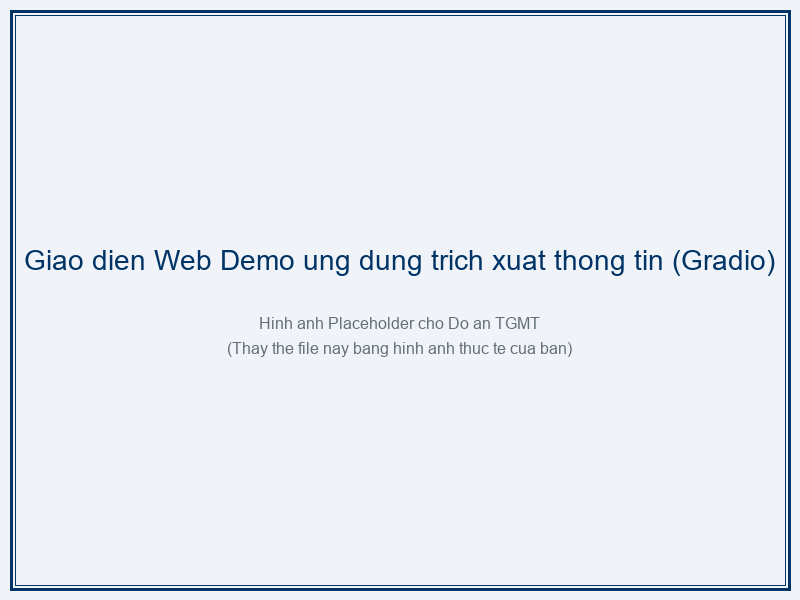
\includegraphics[width=0.9\textwidth]{gradio_demo.png}
  \caption{Giao diện ứng dụng demo Gradio cho trích xuất thông tin biên lai}
  \label{fig:gradio-demo}
\end{figure}

\subsection{Hướng dẫn cài đặt và chạy demo}
\label{appendix:gradio-install}

Để cài đặt và khởi chạy ứng dụng demo, thực hiện các bước sau:

\begin{lstlisting}[language=bash, caption={Cài đặt và chạy ứng dụng Gradio demo}, label={lst:gradio-install}]
# Cai dat project o che do editable
pip install -e .

# Cai dat cac thu vien cho ung dung demo
pip install -r requirements/app.txt

# Khoi chay ung dung demo
python -m receipt_ie.app
\end{lstlisting}

Sau khi chạy lệnh trên, ứng dụng sẽ khởi động tại địa chỉ
\code{http://localhost:7860}. Người dùng có thể truy cập qua trình duyệt web
để sử dụng giao diện demo.


\end{document}
